\documentclass[12pt]{article}

% PACKAGES ---------------------------------------------------------------------
\usepackage[utf8]{inputenc}             % To write accents
\usepackage[english]{babel}             % So LaTeX do proper hyphenation
\usepackage[T1]{fontenc}                % Nicer default font (+ math font)
\usepackage{csquotes}                   % To use \enquote{}
\usepackage{hyperref}                   % Enable links
\usepackage[margin=1in]{geometry}       % To make pretty tables
\usepackage{booktabs}                   % To make pretty tables
\usepackage{tabularx}                   % To make pretty tables
\usepackage{graphicx}                   % Control figures
\usepackage[small,bf,center]{caption}   % Prettier figures
\usepackage{subfig}                     % Prettier figures
\usepackage{setspace}                   % ...
\usepackage{float}                      % To control figures' placement
\usepackage[section]{placeins}          % To control figures' placement
                                        % with \FloatBarrier
\usepackage{indentfirst}                % I like consistency!
\usepackage{relsize}

\begin{document}

\title{
Identifying \emph{large} differences in covariates between groups\\[0.2em]\footnotesize{}Online appendix for \emph{Expecting to get it: An Endowment Effect for Information}}


\author{Tabaré Capitán
        \and
        Linda Thunström
        \and
        Klaas van ‘t Veld
          \\ \small{Department of Economics, University of Wyoming}
        \and
        Jonas Nordström
          \\ \small{Lund University and University of Copenhagen}
        }
\maketitle

\thispagestyle{empty}   % Suppress page number (must be under \maketitle)

\clearpage

\tableofcontents

\clearpage

\section{Low baseline (groups A and B) vs high baseline (groups C and D)}

In this section we compare the group of participants who received menus without calorie information in their hypothetical choices (groups A and B) to the group of participants who received menus with calorie information in their hypothetical choices (groups C and D). The multivariate difference in normalized means is 0.645.

\subsection{Demographics}

\begin{itemize}
  \item \textbf{Female}: No \emph{large} difference.

  \item \textbf{Age}: No \emph{large} difference.

  \item \textbf{College}: No \emph{large} difference.

  \item \textbf{Expenses}: No \emph{large} difference.

  \item \textbf{Income}: No \emph{large} difference.

  \item \textbf{Weight description}: No \emph{large} difference.

  \item \textbf{BMI}: No \emph{large} difference.
\end{itemize}

\begin{figure}[ht]
  \caption{Balance in demographic characteristics \\ (groups A and B vs groups C and D)}\label{fig:group1_demographics}
  \begin{center}
  {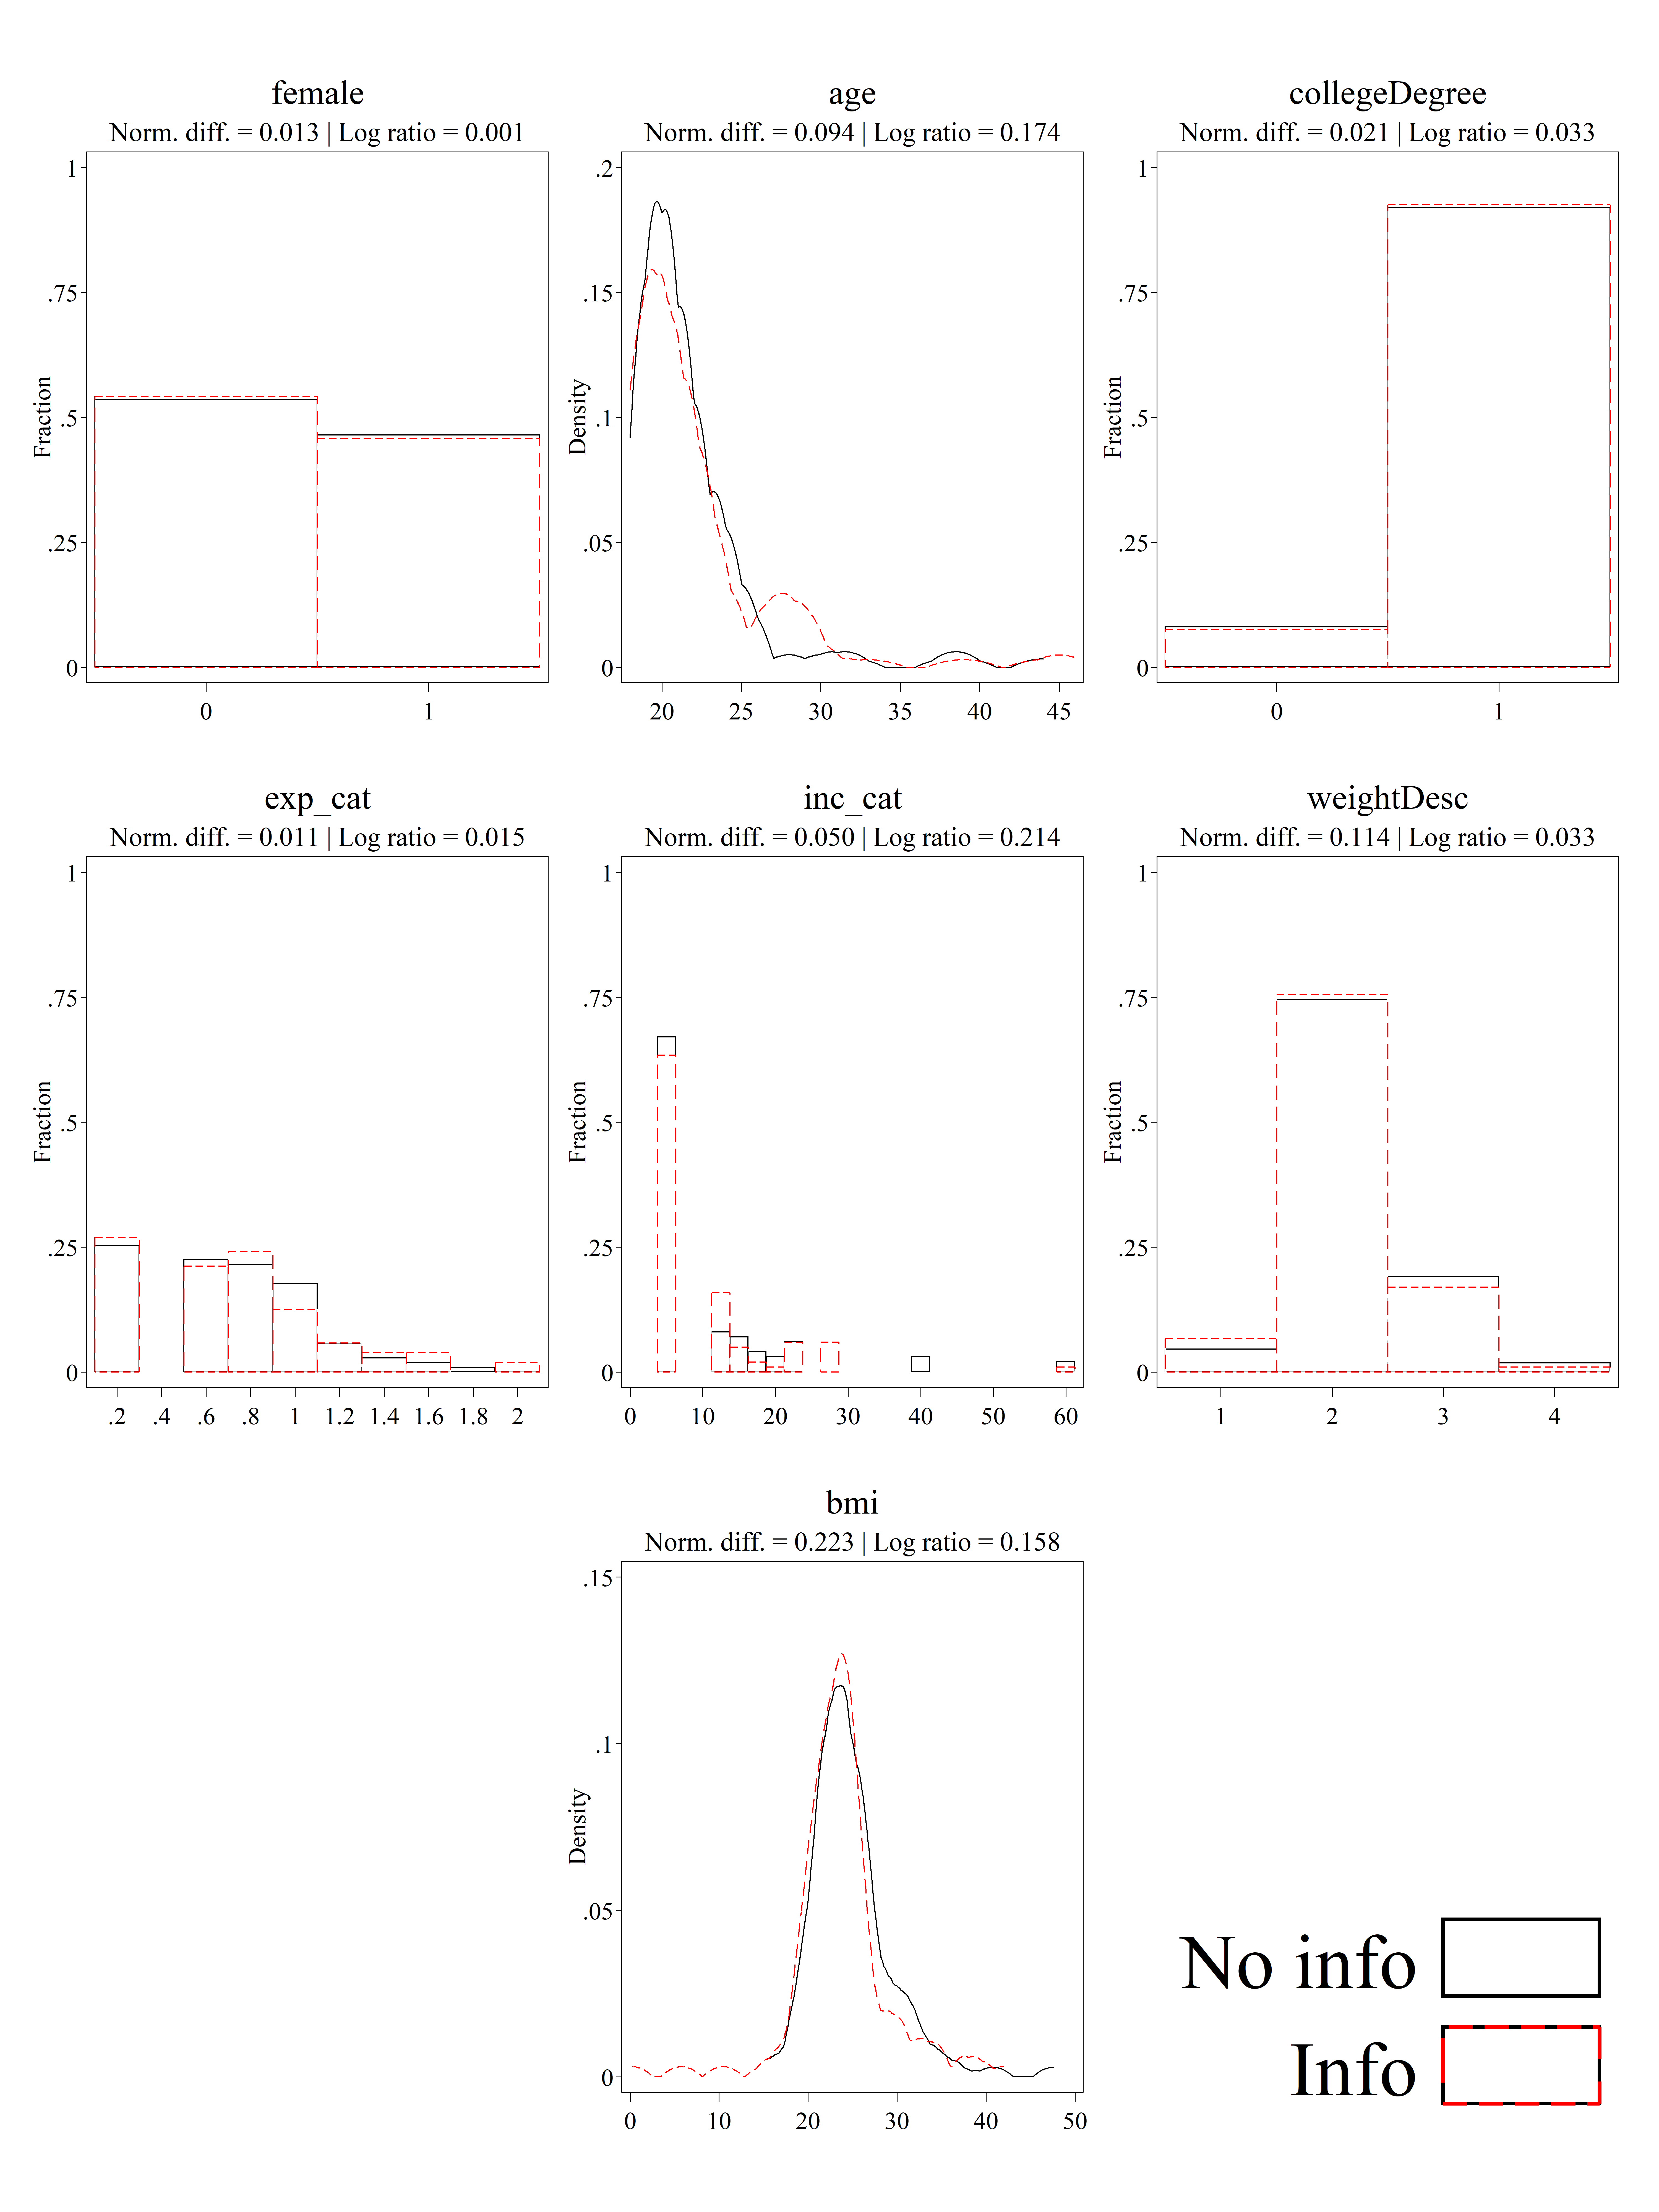
\includegraphics[width=1\textwidth]{./figures/covDifExp_demographics.png}}
  \end{center}
\end{figure}

\FloatBarrier

\clearpage

\subsection{Attitudes}

\begin{itemize}
  \item \textbf{Risk preferences}: \emph{Large} difference.
  Normalized difference over $0.25$. The difference is driven by differences in the share of participants of each group at both ends of the distribution.

  \item \textbf{Discount factor $\delta$}: No \emph{large} difference.

  \item \textbf{Present-bias $\beta$}: No \emph{large} difference.
  High log ratio driven by outliers that likely reflect mistakes.

  \item \textbf{Food-self control}: No \emph{large} difference.

  \item \textbf{Hunger level}: No \emph{large} difference.
\end{itemize}

\begin{figure}[ht]
  \caption{Balance in demographic characteristics \\ (groups A and B vs groups C and D)}\label{fig:group1_attitudes}
  \begin{center}
  {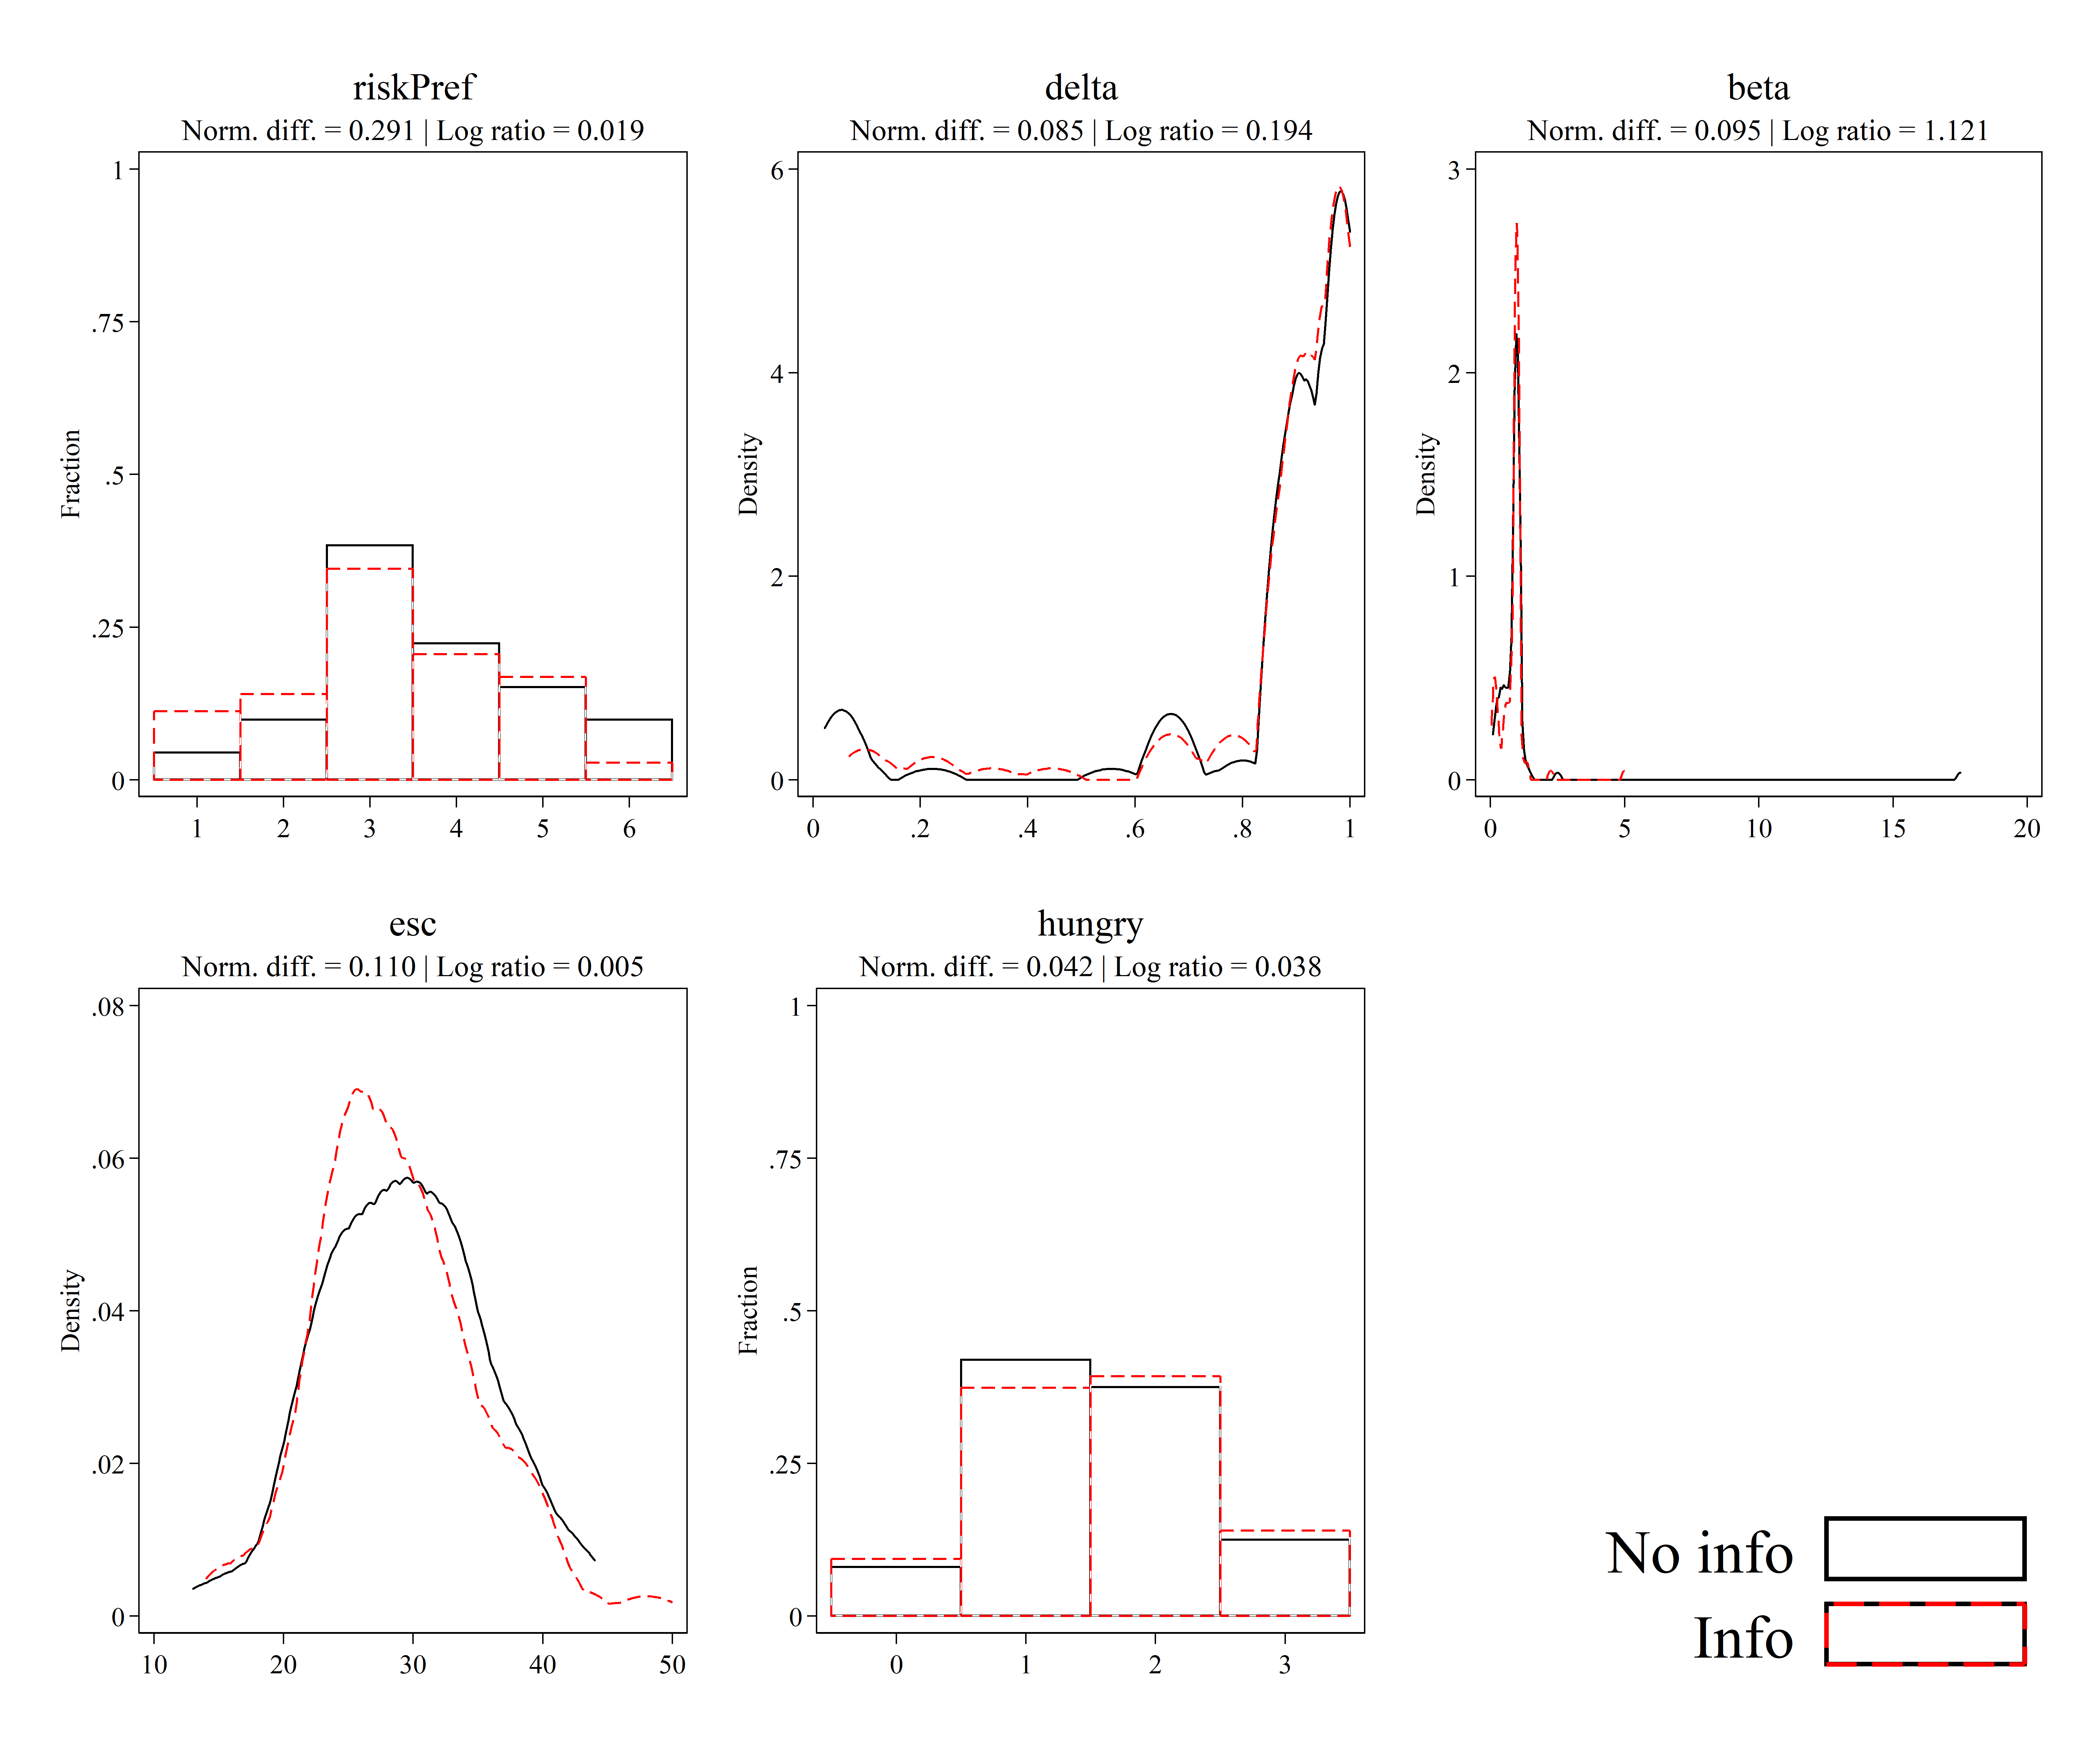
\includegraphics[width=1\textwidth]{./figures/covDifExp_attitudes.png}}
  \end{center}
\end{figure}

\FloatBarrier

\clearpage

\subsection{Health status and perceptions}

\begin{itemize}
  \item \textbf{Health assessment}: No \emph{large} difference.

  \item \textbf{Would benefit from eating healthier}: No \emph{large} difference.

  \item \textbf{Wish could eat healthier at home}: No \emph{large} difference.

  \item \textbf{Wish could eat healthier out}: No \emph{large} difference.

  \item \textbf{Importance of eating healthy food}: No \emph{large} difference.

  \item \textbf{Importance of exercising regularly}: No \emph{large} difference.

  \item \textbf{Importance of healthy body weight}: No \emph{large} difference.
\end{itemize}

\begin{figure}[ht]
  \caption{Balance in demographic characteristics \\ (groups A and B vs groups C and D)}\label{fig:group1_health}
  \begin{center}
  {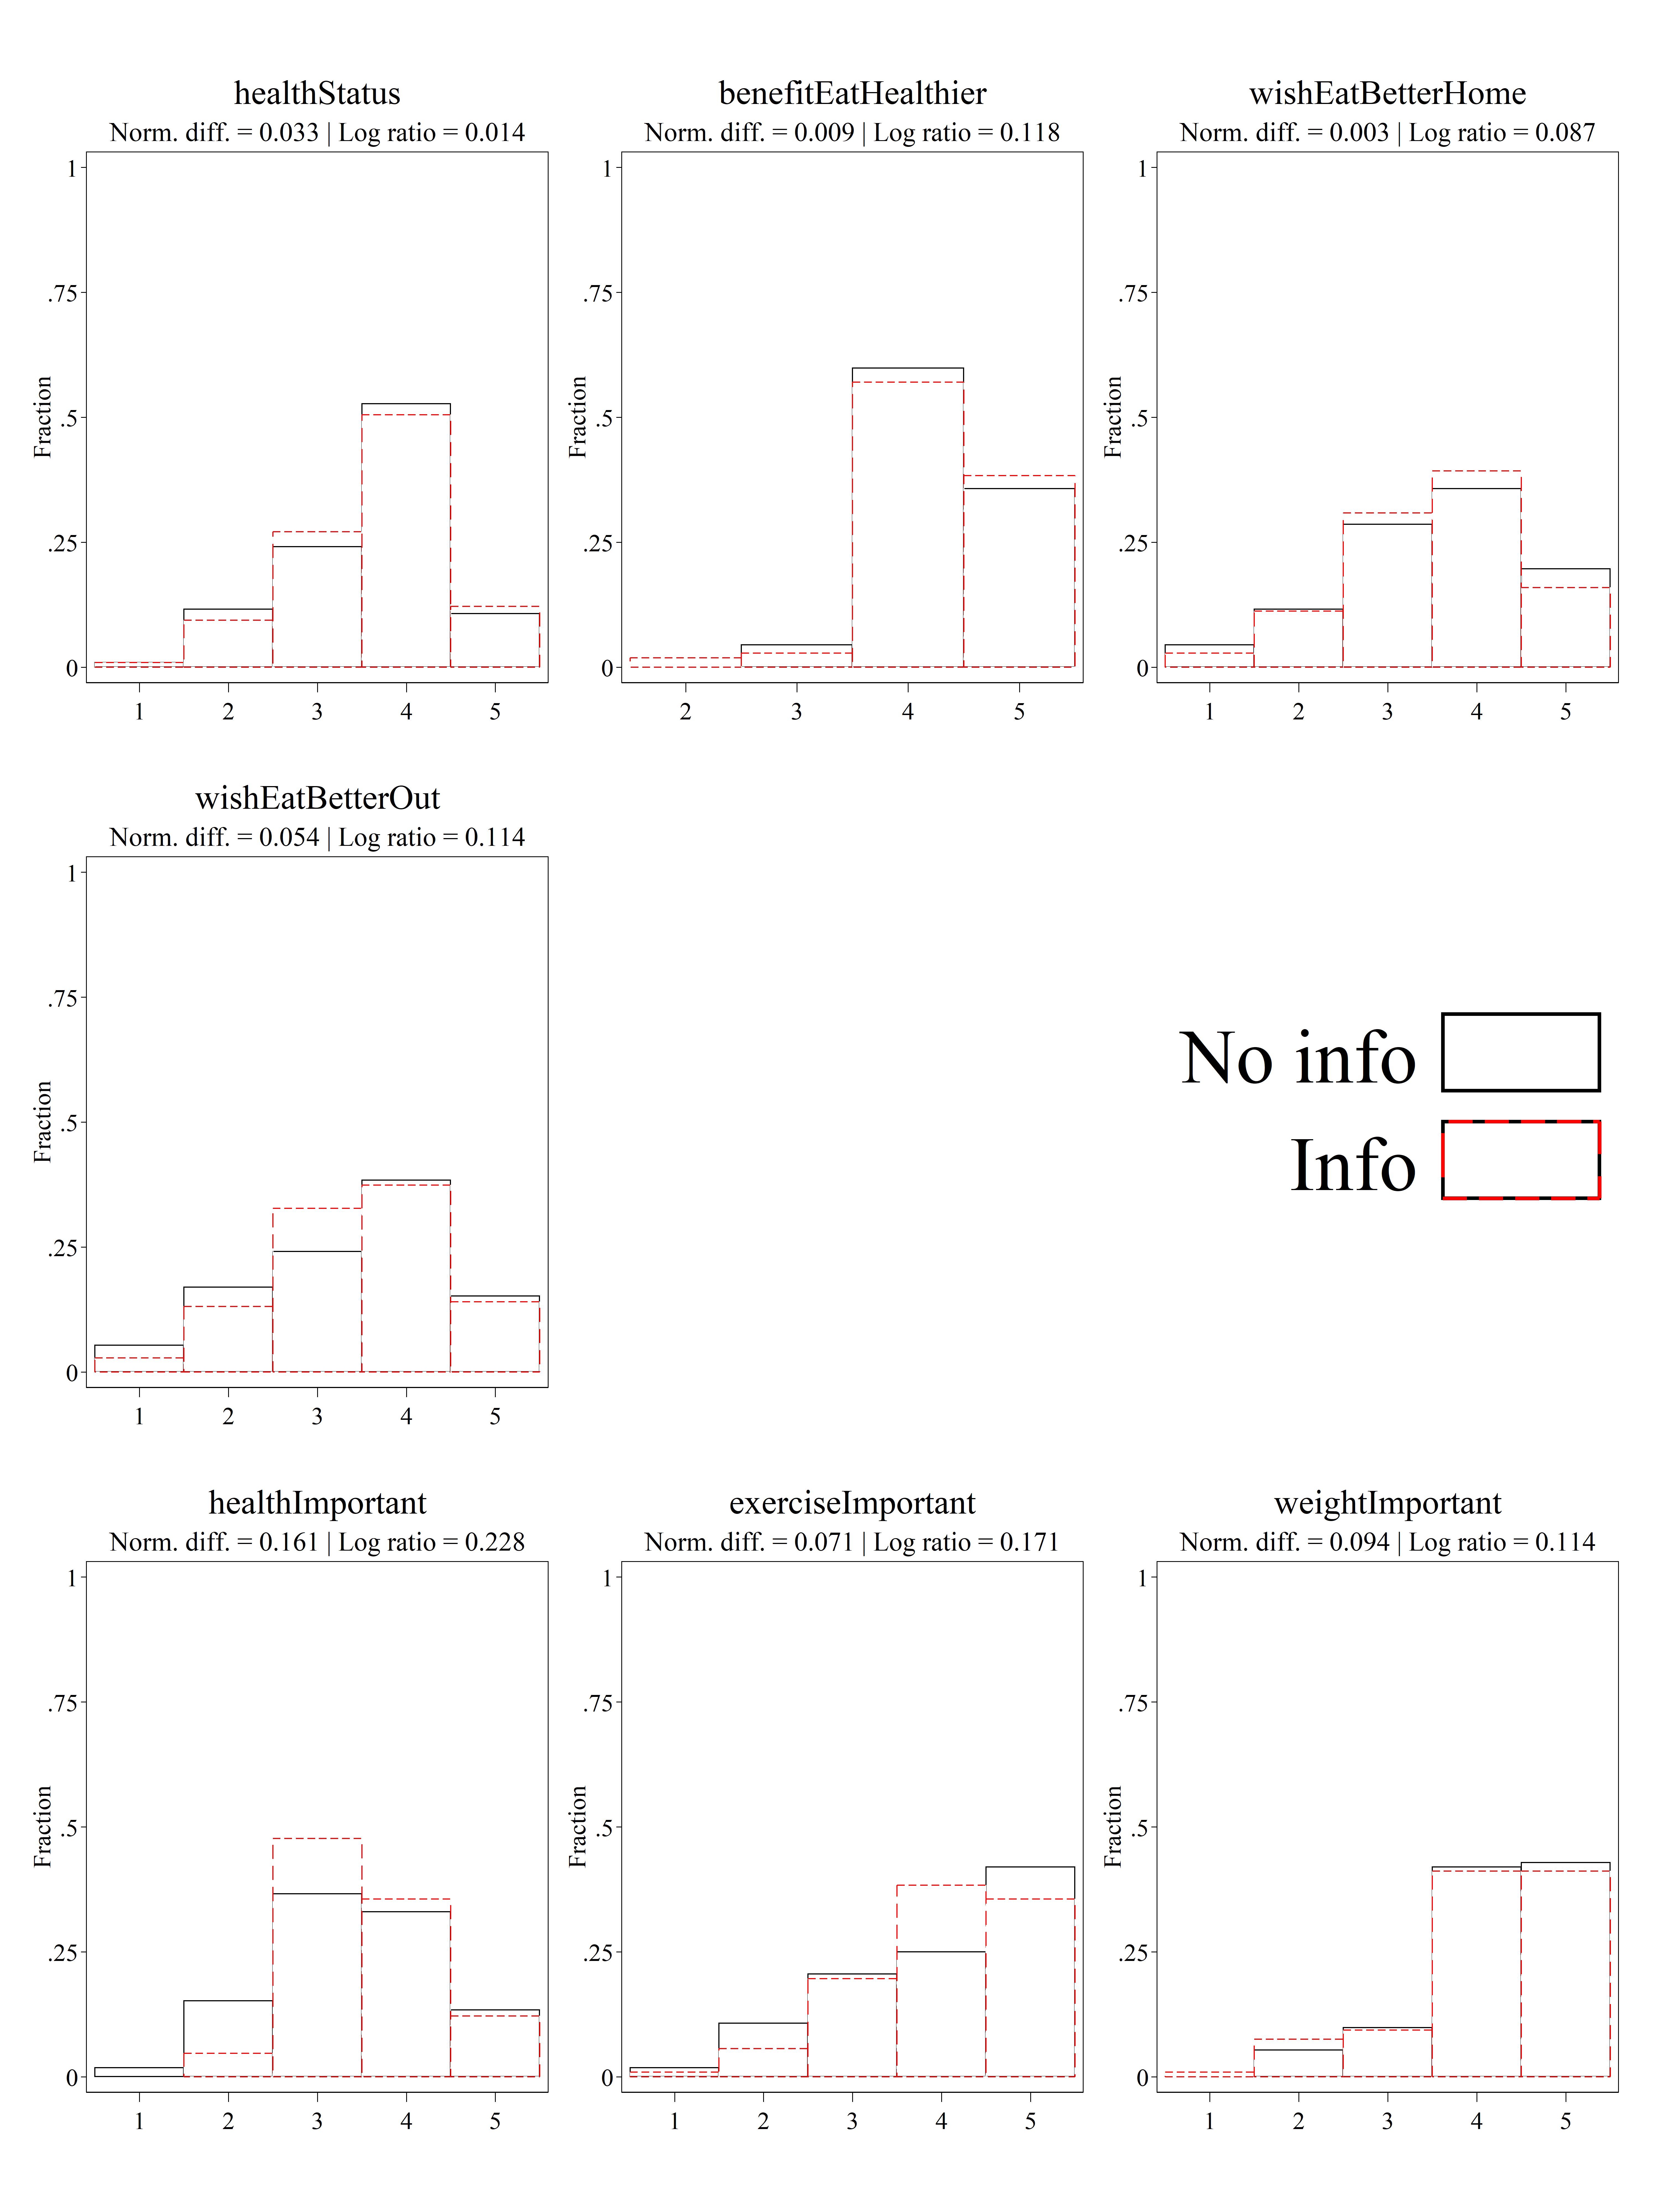
\includegraphics[width=1\textwidth]{./figures/covDifExp_health.png}}
  \end{center}
\end{figure}

\FloatBarrier

\clearpage

\subsection{Knowledge of calorie information}

\begin{itemize}
  \item \textbf{Knows calorie needs}: No \emph{large} difference.

  \item \textbf{Experience with calorie information}: No \emph{large} difference.

  \item \textbf{Frequency visits to chain restaurants}: No \emph{large} difference.
\end{itemize}

\begin{figure}[ht]
  \caption{Balance in demographic characteristics \\ (groups A and B vs groups C and D)}\label{fig:group1_calorie}
  \begin{center}
  {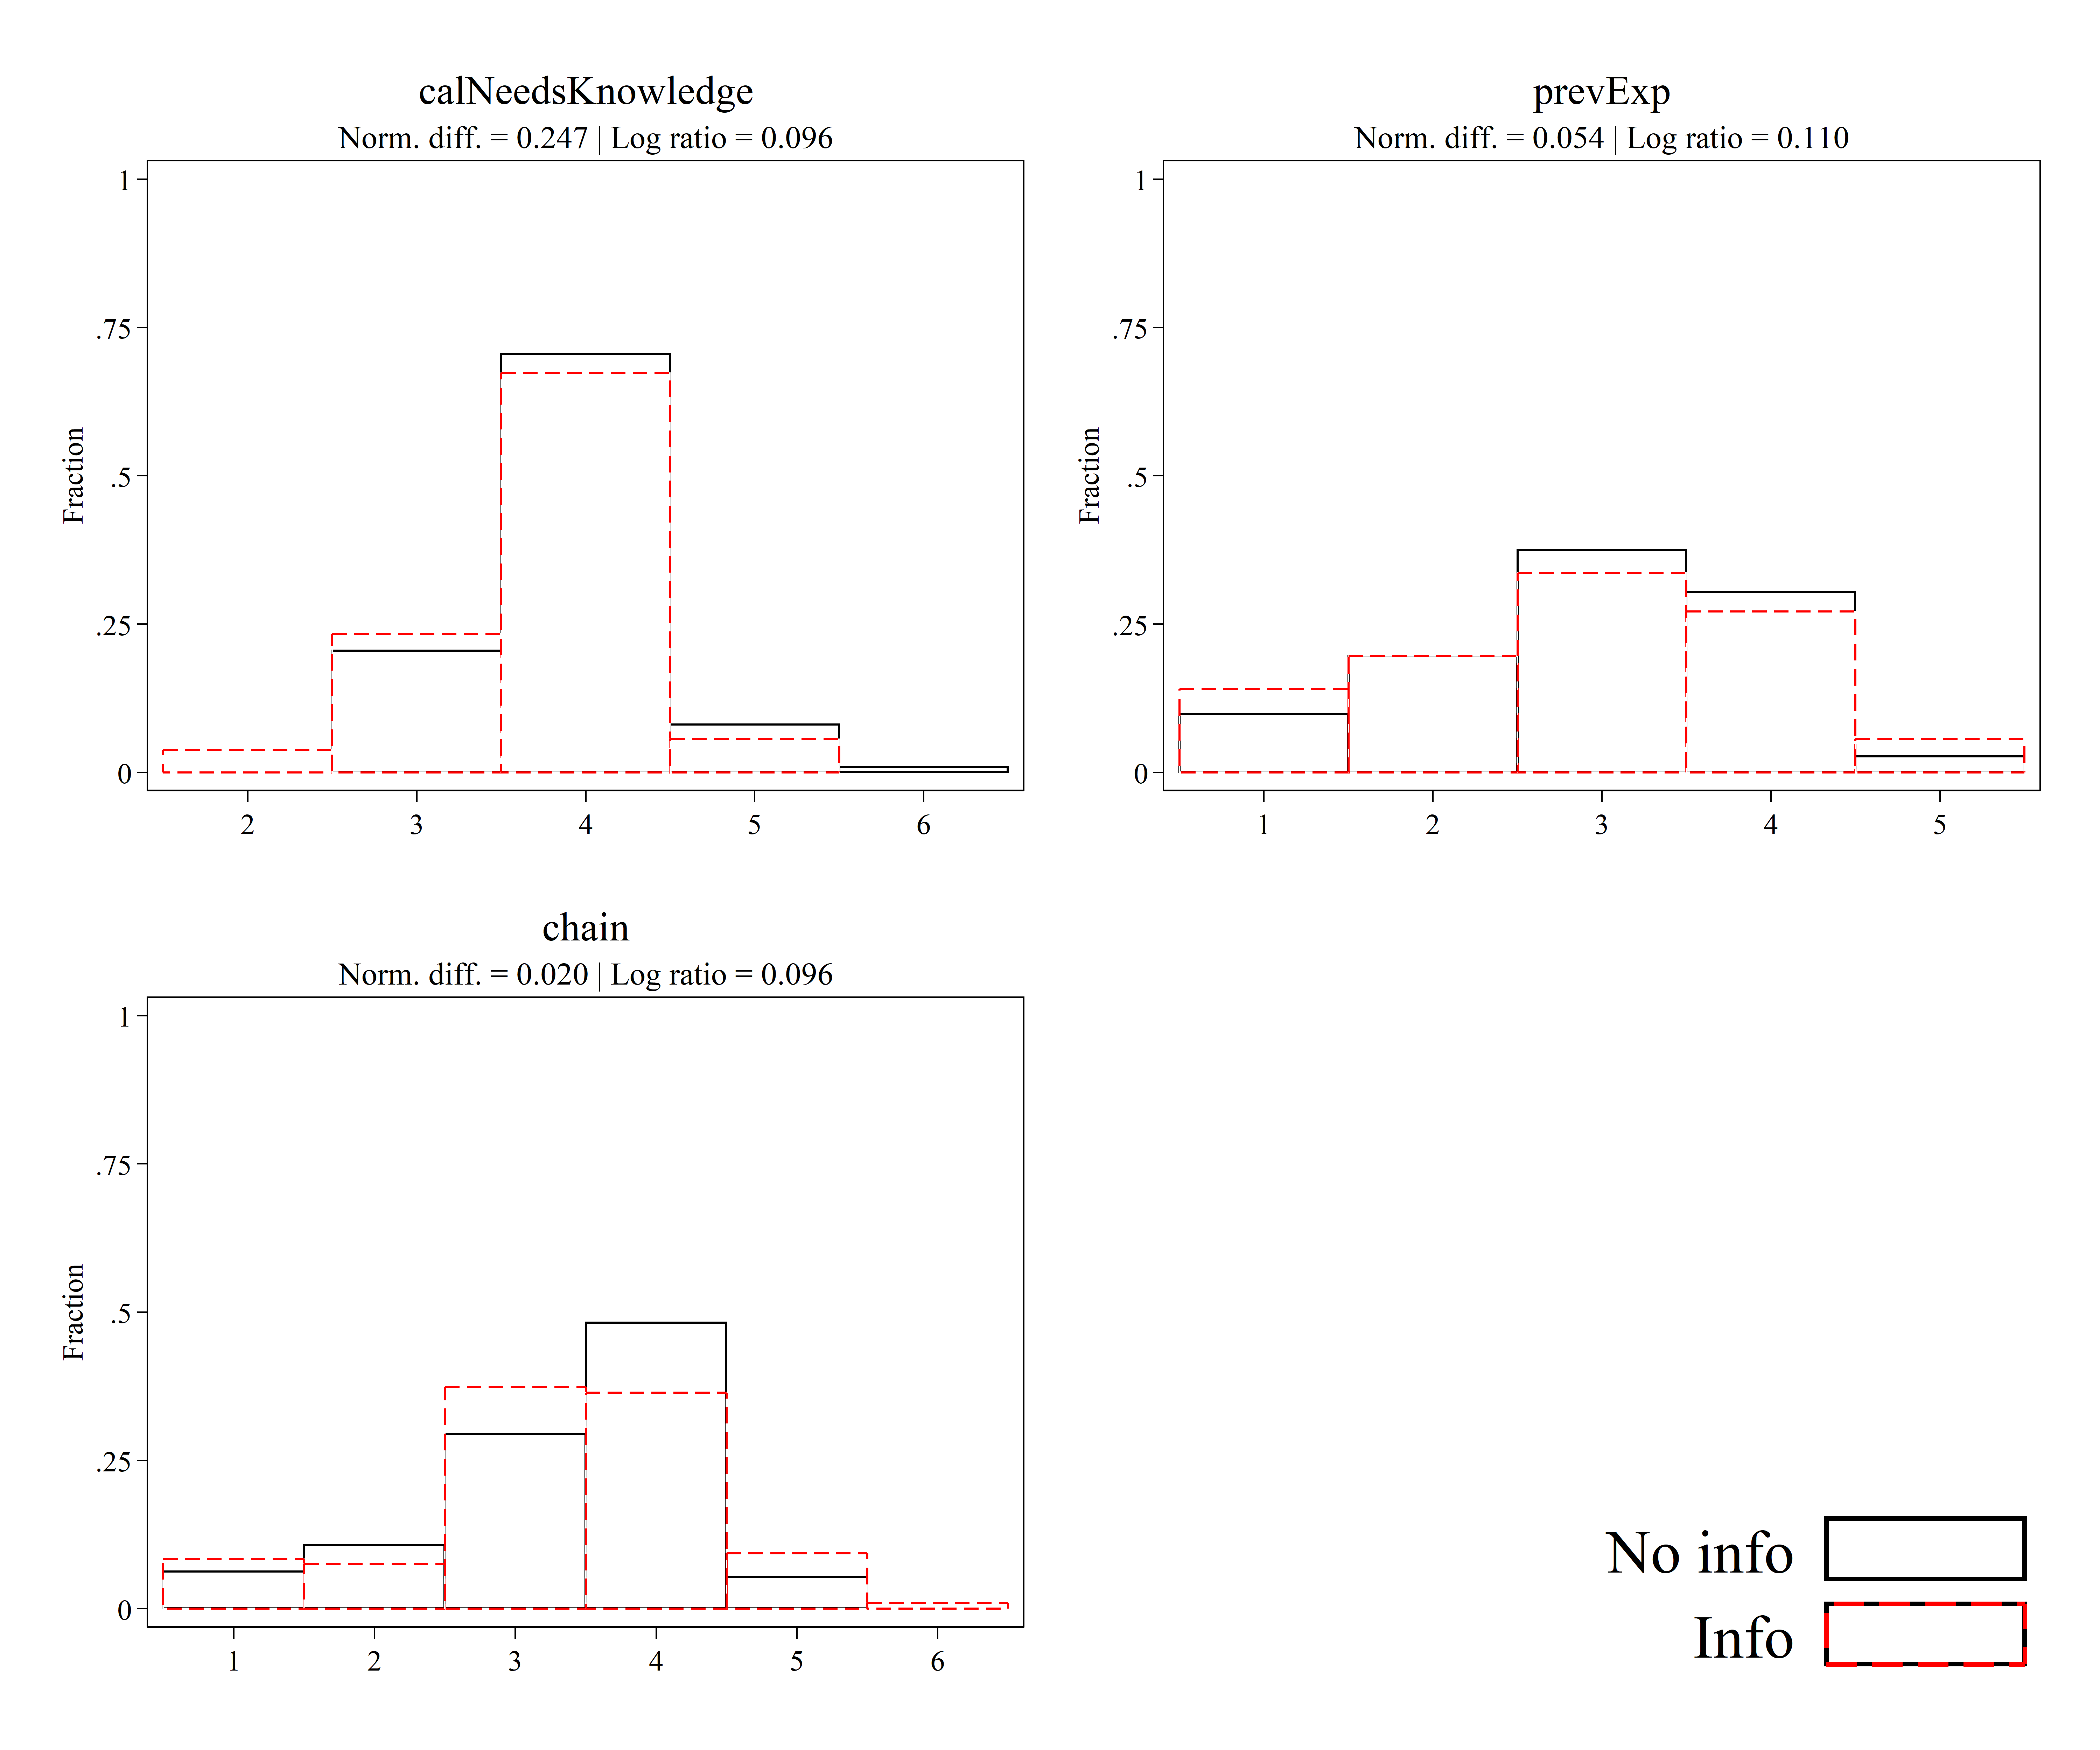
\includegraphics[width=1\textwidth]{./figures/covDifExp_calorieKnow.png}}
  \end{center}
\end{figure}

\FloatBarrier

\clearpage

% ------------------------------------------------------------------------------

\section{Low baseline: group A vs group B}

Within participants who received a menu without calorie information for their hypothetical choices (low baseline, groups A and B): The group if participants who received a menu without calorie information for their real choice (group A) and the group of participants who received a menu with covered calorie information for their real choice (group B). The multivariate difference in normalized means is $0.94$.

\subsection{Demographics}

\begin{itemize}
  \item \textbf{Female}: No \emph{large} difference.

  \item \textbf{Age}: No \emph{large} difference.
  The normalized difference of variances is 0.68, but this difference is driven by 3 outliers in the no info group (38, 39, and 44 years old). Without the outliers, the normalized difference in means is .15 standard deviations and the normalized difference in variances is 0.03.

  \item \textbf{College}: \emph{Large} difference.

  \item \textbf{Expenses}: \emph{Large} difference.

  \item \textbf{Income}: No \emph{large} difference.
  High log ratio driven by one outlier.

  \item \textbf{Weight description}: No \emph{large} difference.

  \item \textbf{BMI}: No \emph{large} difference.
\end{itemize}

\begin{figure}[ht]
  \caption{Balance in demographic characteristics \\ (group A vs B)}\label{fig:group2_demographics}
  \begin{center}
  {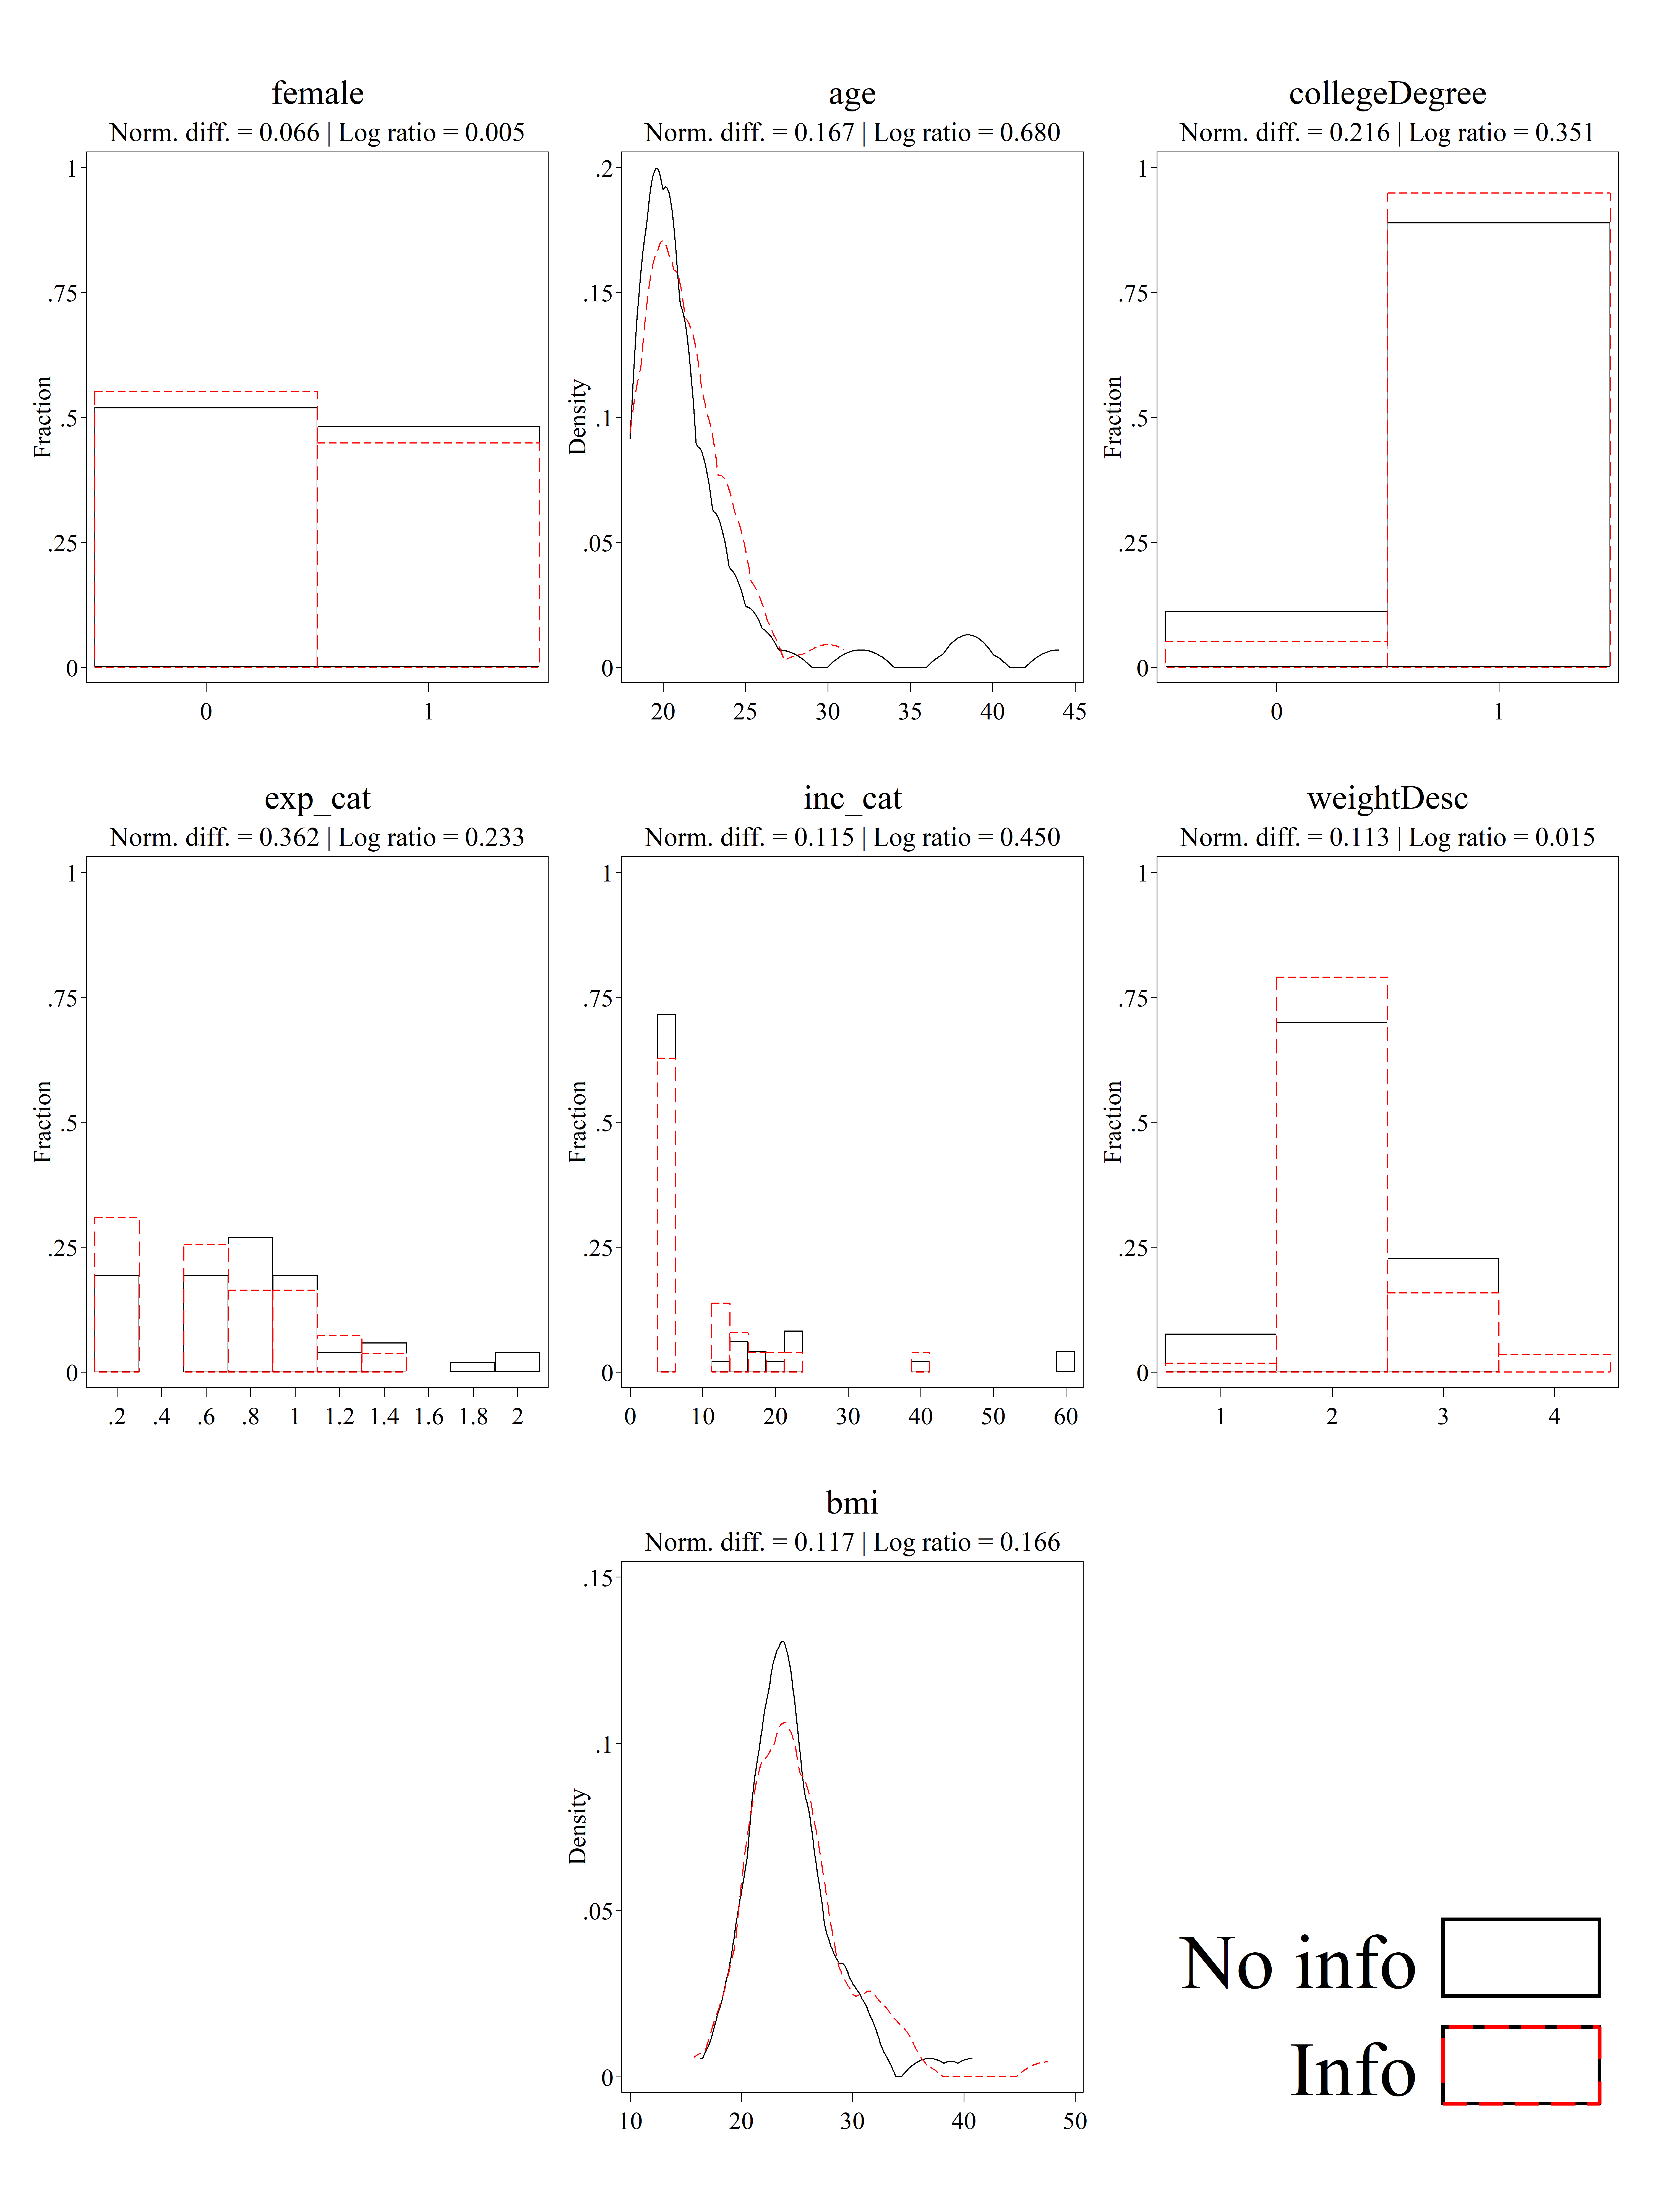
\includegraphics[width=1\textwidth]{./figures/covDifTreat_0_demographics.png}}
  \end{center}
\end{figure}

\FloatBarrier

\clearpage

\subsection{Attitudes}

\begin{itemize}
  \item \textbf{Risk preferences}: \emph{Large} difference.
  Despite having a normalized difference in means of only 0.19 standard deviations and a normalized difference in variance of only 0.1, we identify the difference as large because the share of participants in the no info group exceeds the share in the info group by 9.64 pp in the most extreme category (i.e., stronger risk preferences).

  \item \textbf{Discount factor $\delta$}: No \emph{large} difference.

  \item \textbf{Present-bias $\beta$}: \emph{Large} difference.

  \item \textbf{Food-self control}: No \emph{large} difference.

  \item \textbf{Hunger level}: No \emph{large} difference.
\end{itemize}

\begin{figure}[ht]
  \caption{Balance in demographic characteristics \\ (group A vs B)}\label{fig:group2_attitudes}
  \begin{center}
  {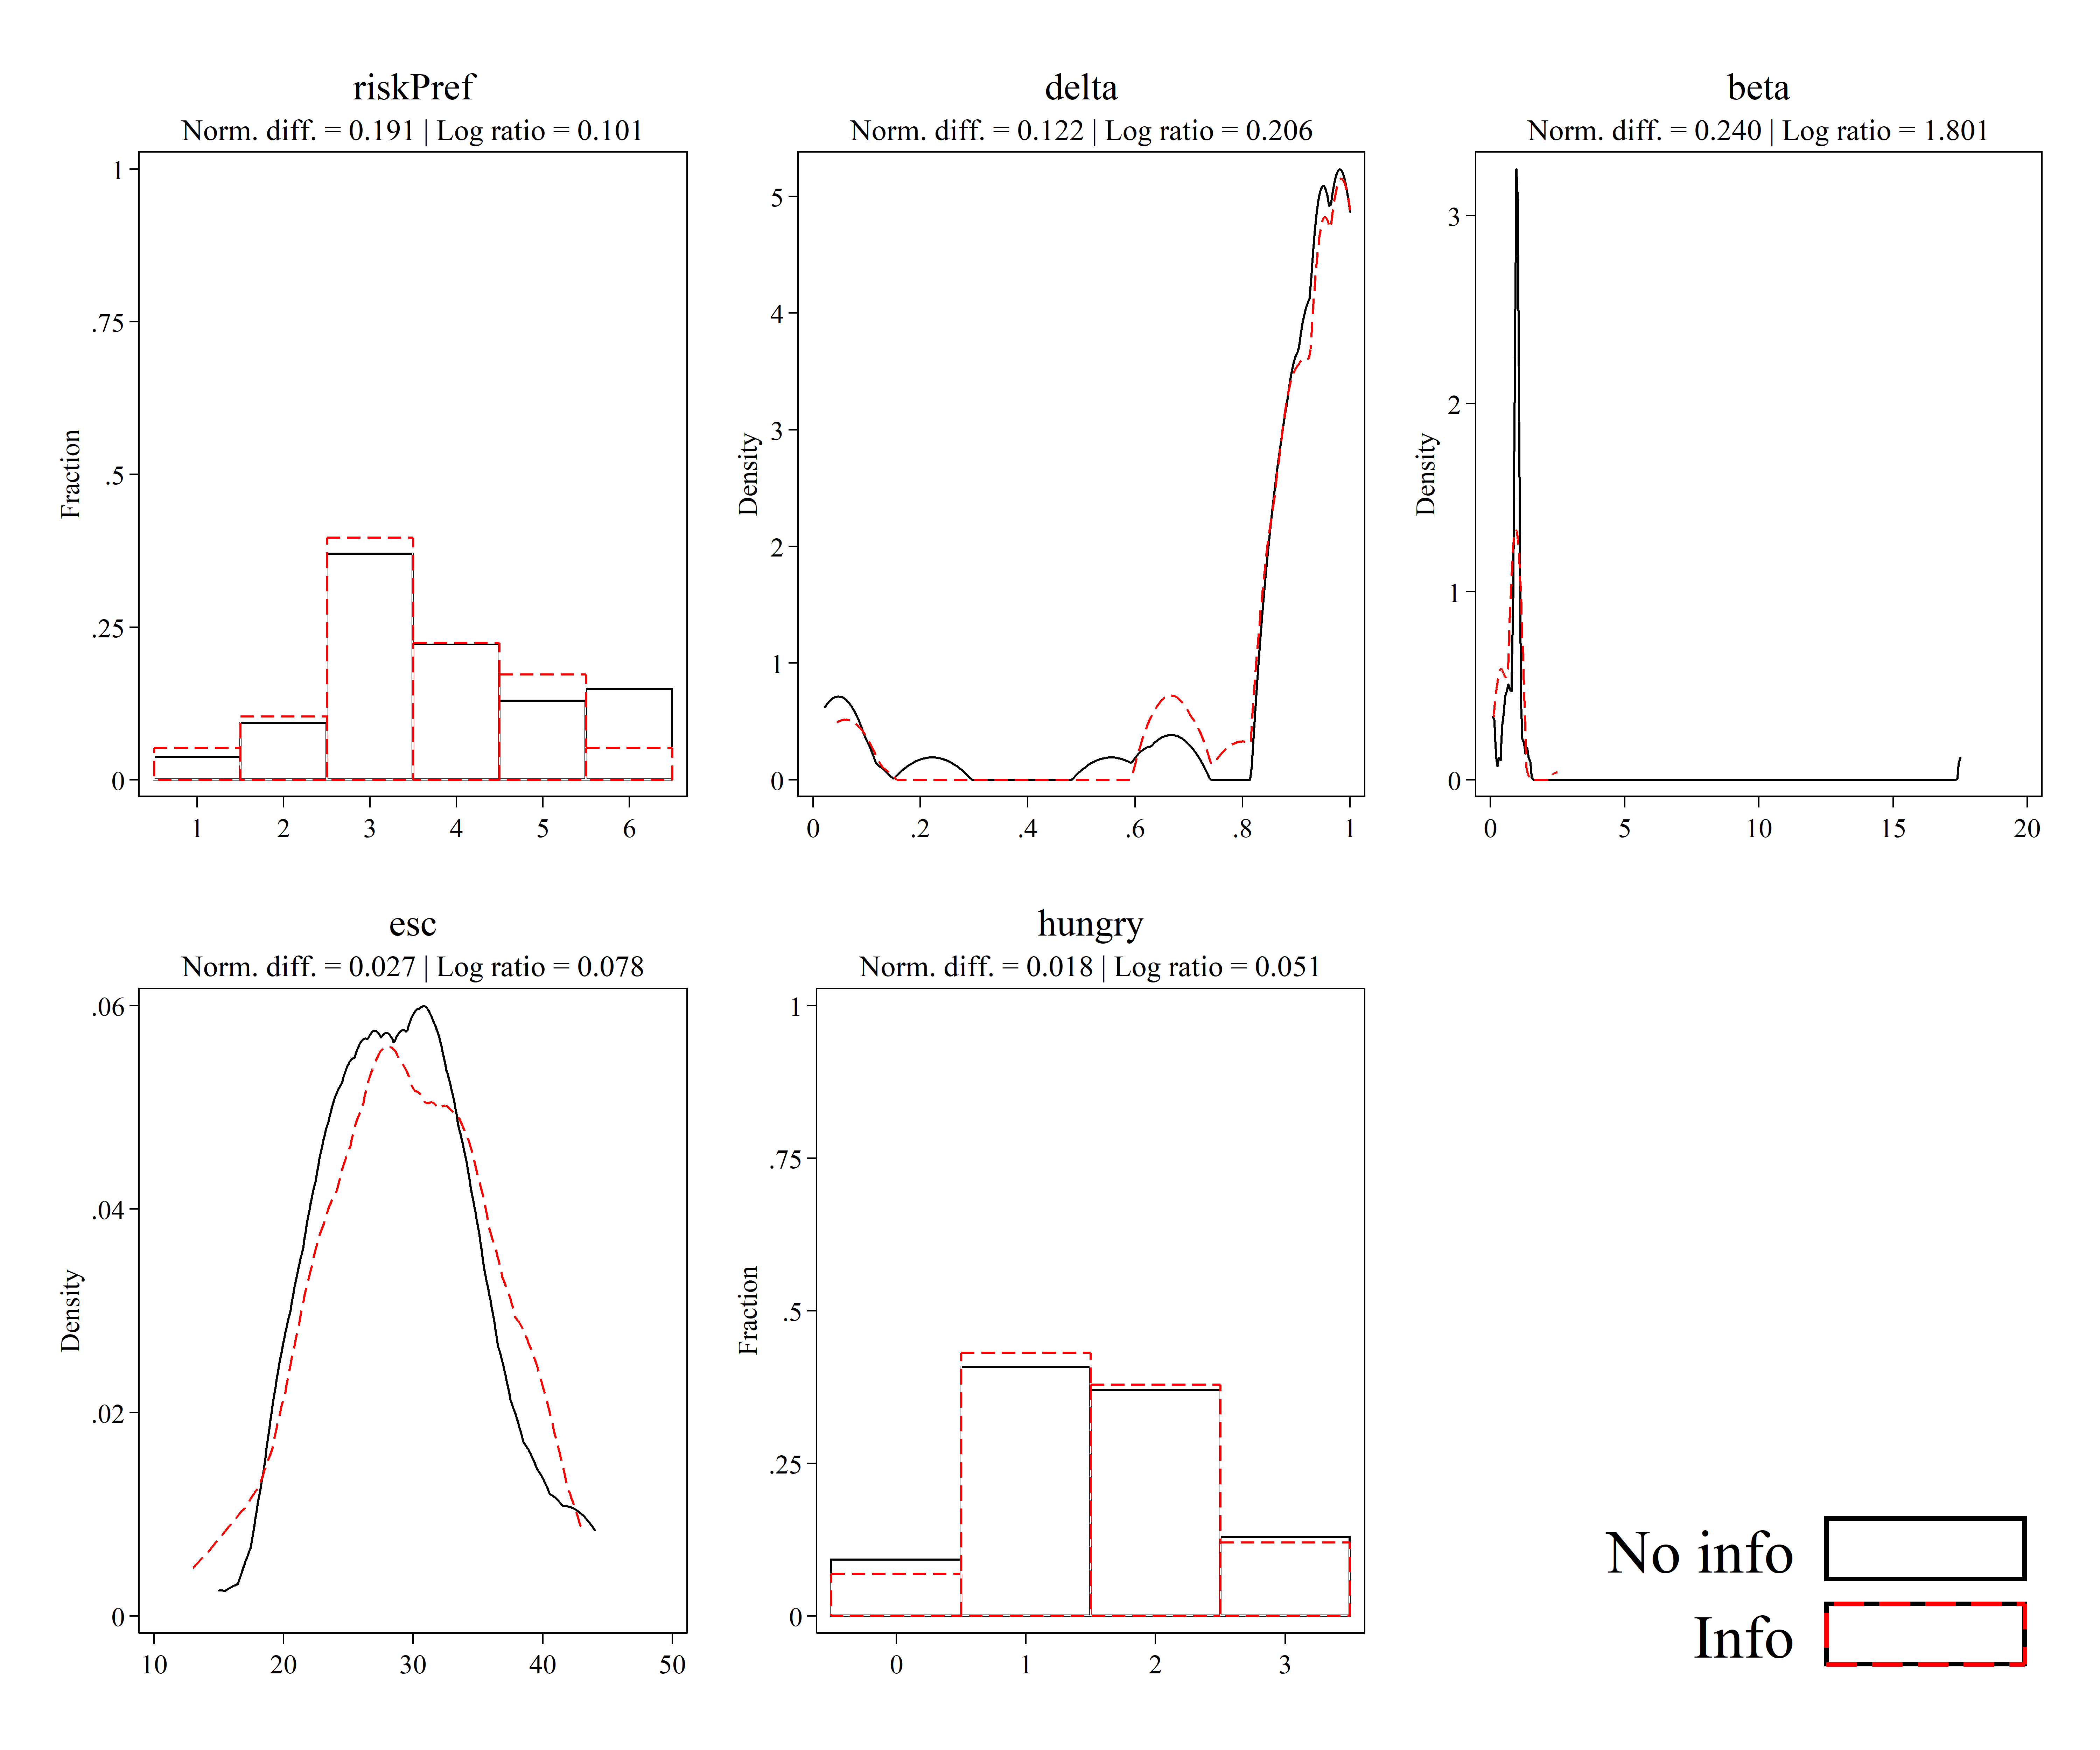
\includegraphics[width=1\textwidth]{./figures/covDifTreat_0_attitudes.png}}
  \end{center}
\end{figure}

\FloatBarrier

\clearpage

\subsection{Health status and perceptions}

\begin{itemize}
  \item \textbf{Health assessment}: \emph{Large} difference.
  Despite a low normalized difference in means, the histogram shows that the endowed group reports better health than the other group. The differences in shares responding 3 and 4 somewhat mask the difference.

  \item \textbf{Would benefit from eating healthier}: No \emph{large} difference.

  \item \textbf{Wish could eat healthier at home}: No \emph{large} difference.

  \item \textbf{Wish could eat healthier out}: \emph{Large} difference.

  \item \textbf{Importance of eating healthy food}: No \emph{large} difference.
  The normalized difference in means is just above the threshold given by the general rule, but we think that the interpretation between 1 and 2, and between 4 and 5, is problematic. If we assume only a positive (4 and 5), neutral (3), and negative (1 and 2) interpretation, the covariates seem more balanced.

  \item \textbf{Importance of exercising regularly}: No \emph{large} difference.

  \item \textbf{Importance of healthy body weight}: No \emph{large} difference.
\end{itemize}

\begin{figure}[ht]
  \caption{Balance in demographic characteristics \\ (groups A and B vs groups C and D)}\label{fig:group2_health}
  \begin{center}
  {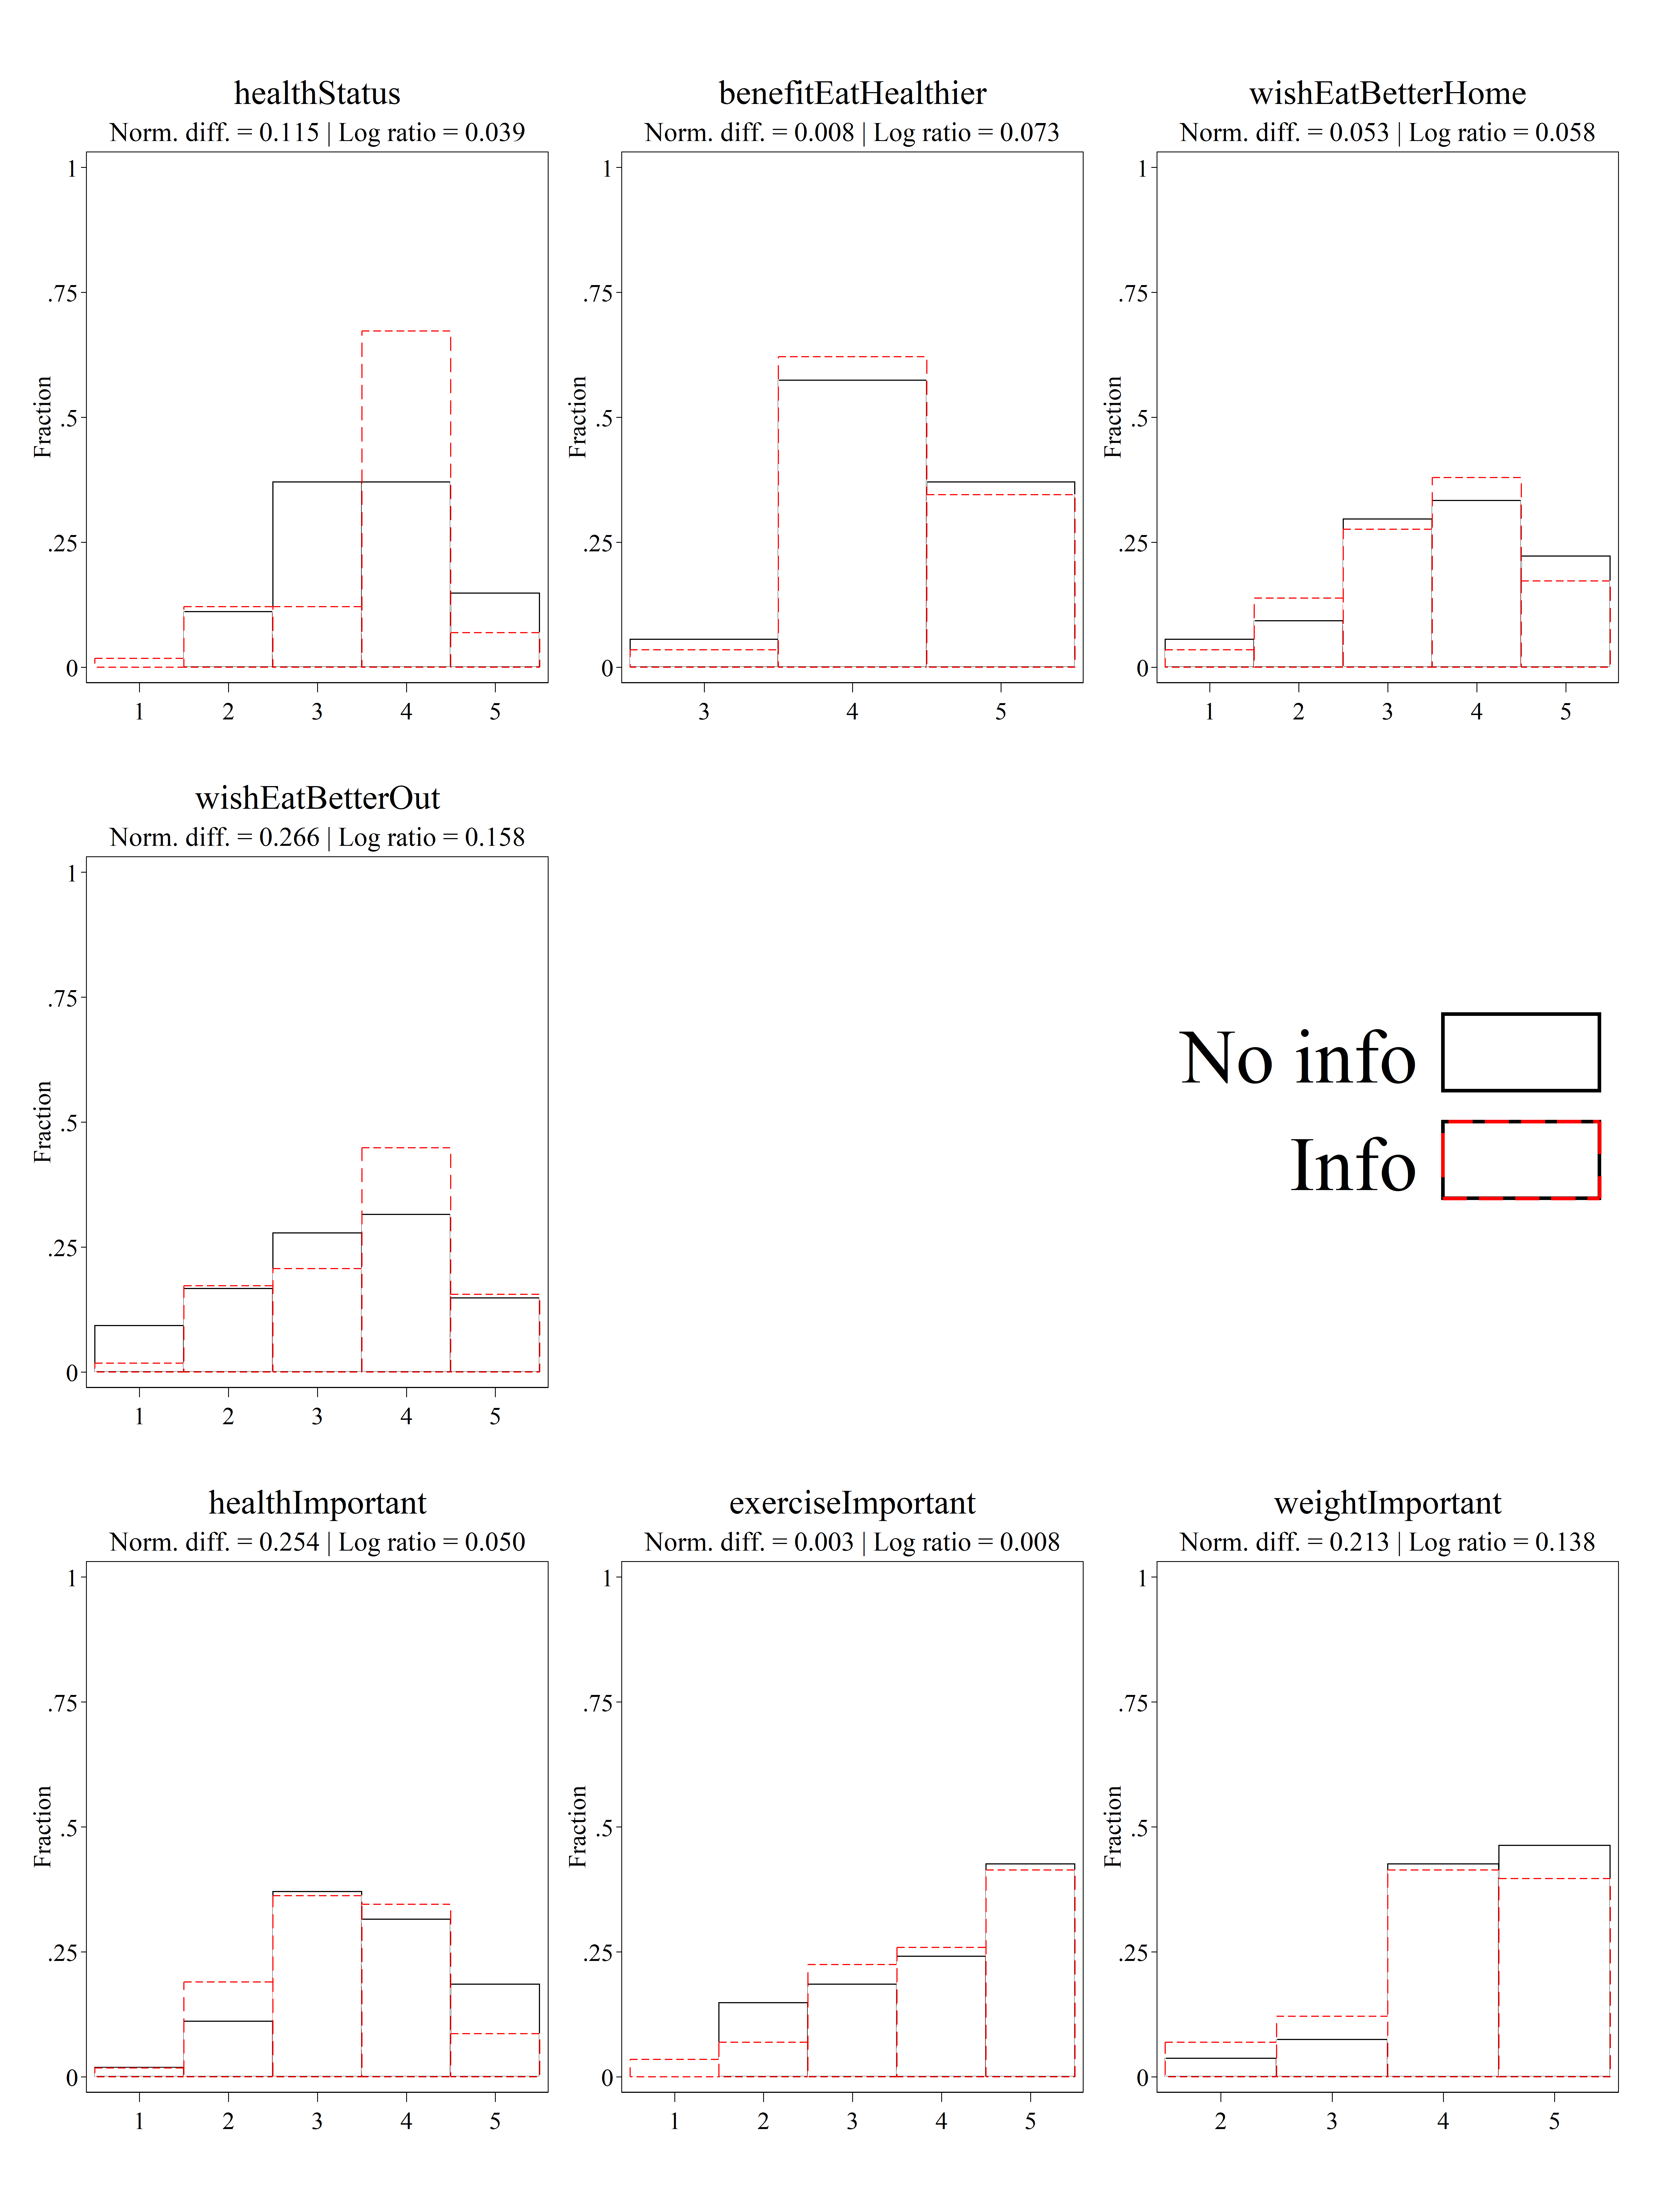
\includegraphics[width=1\textwidth]{./figures/covDifTreat_0_health.png}}
  \end{center}
\end{figure}

\FloatBarrier

\clearpage

\subsection{Knowledge of calorie information}

\begin{itemize}
  \item \textbf{Knows calorie needs}: \emph{Large} difference.
  The normalized difference in means is low, but the share of the endowed group that answer 4 (i.e., 2500 calorie) is 7.5 pp higher than the other group. In other words, a significantly higher share of people in the endowed group responded correctly to the question of daily calorie needs.

  \item \textbf{Experience with calorie information}: \emph{Large} difference.
  Again, the first two moments of the distribution do not reveal differences, but the histogram shows a marked difference between groups in the way they respond 2 and 4.

  \item \textbf{Frequency visits to chain restaurants}: No \emph{large} difference.
\end{itemize}

\begin{figure}[ht]
  \caption{Balance in demographic characteristics \\ (groups A and B vs groups C and D)}\label{fig:group2_calorie}
  \begin{center}
  {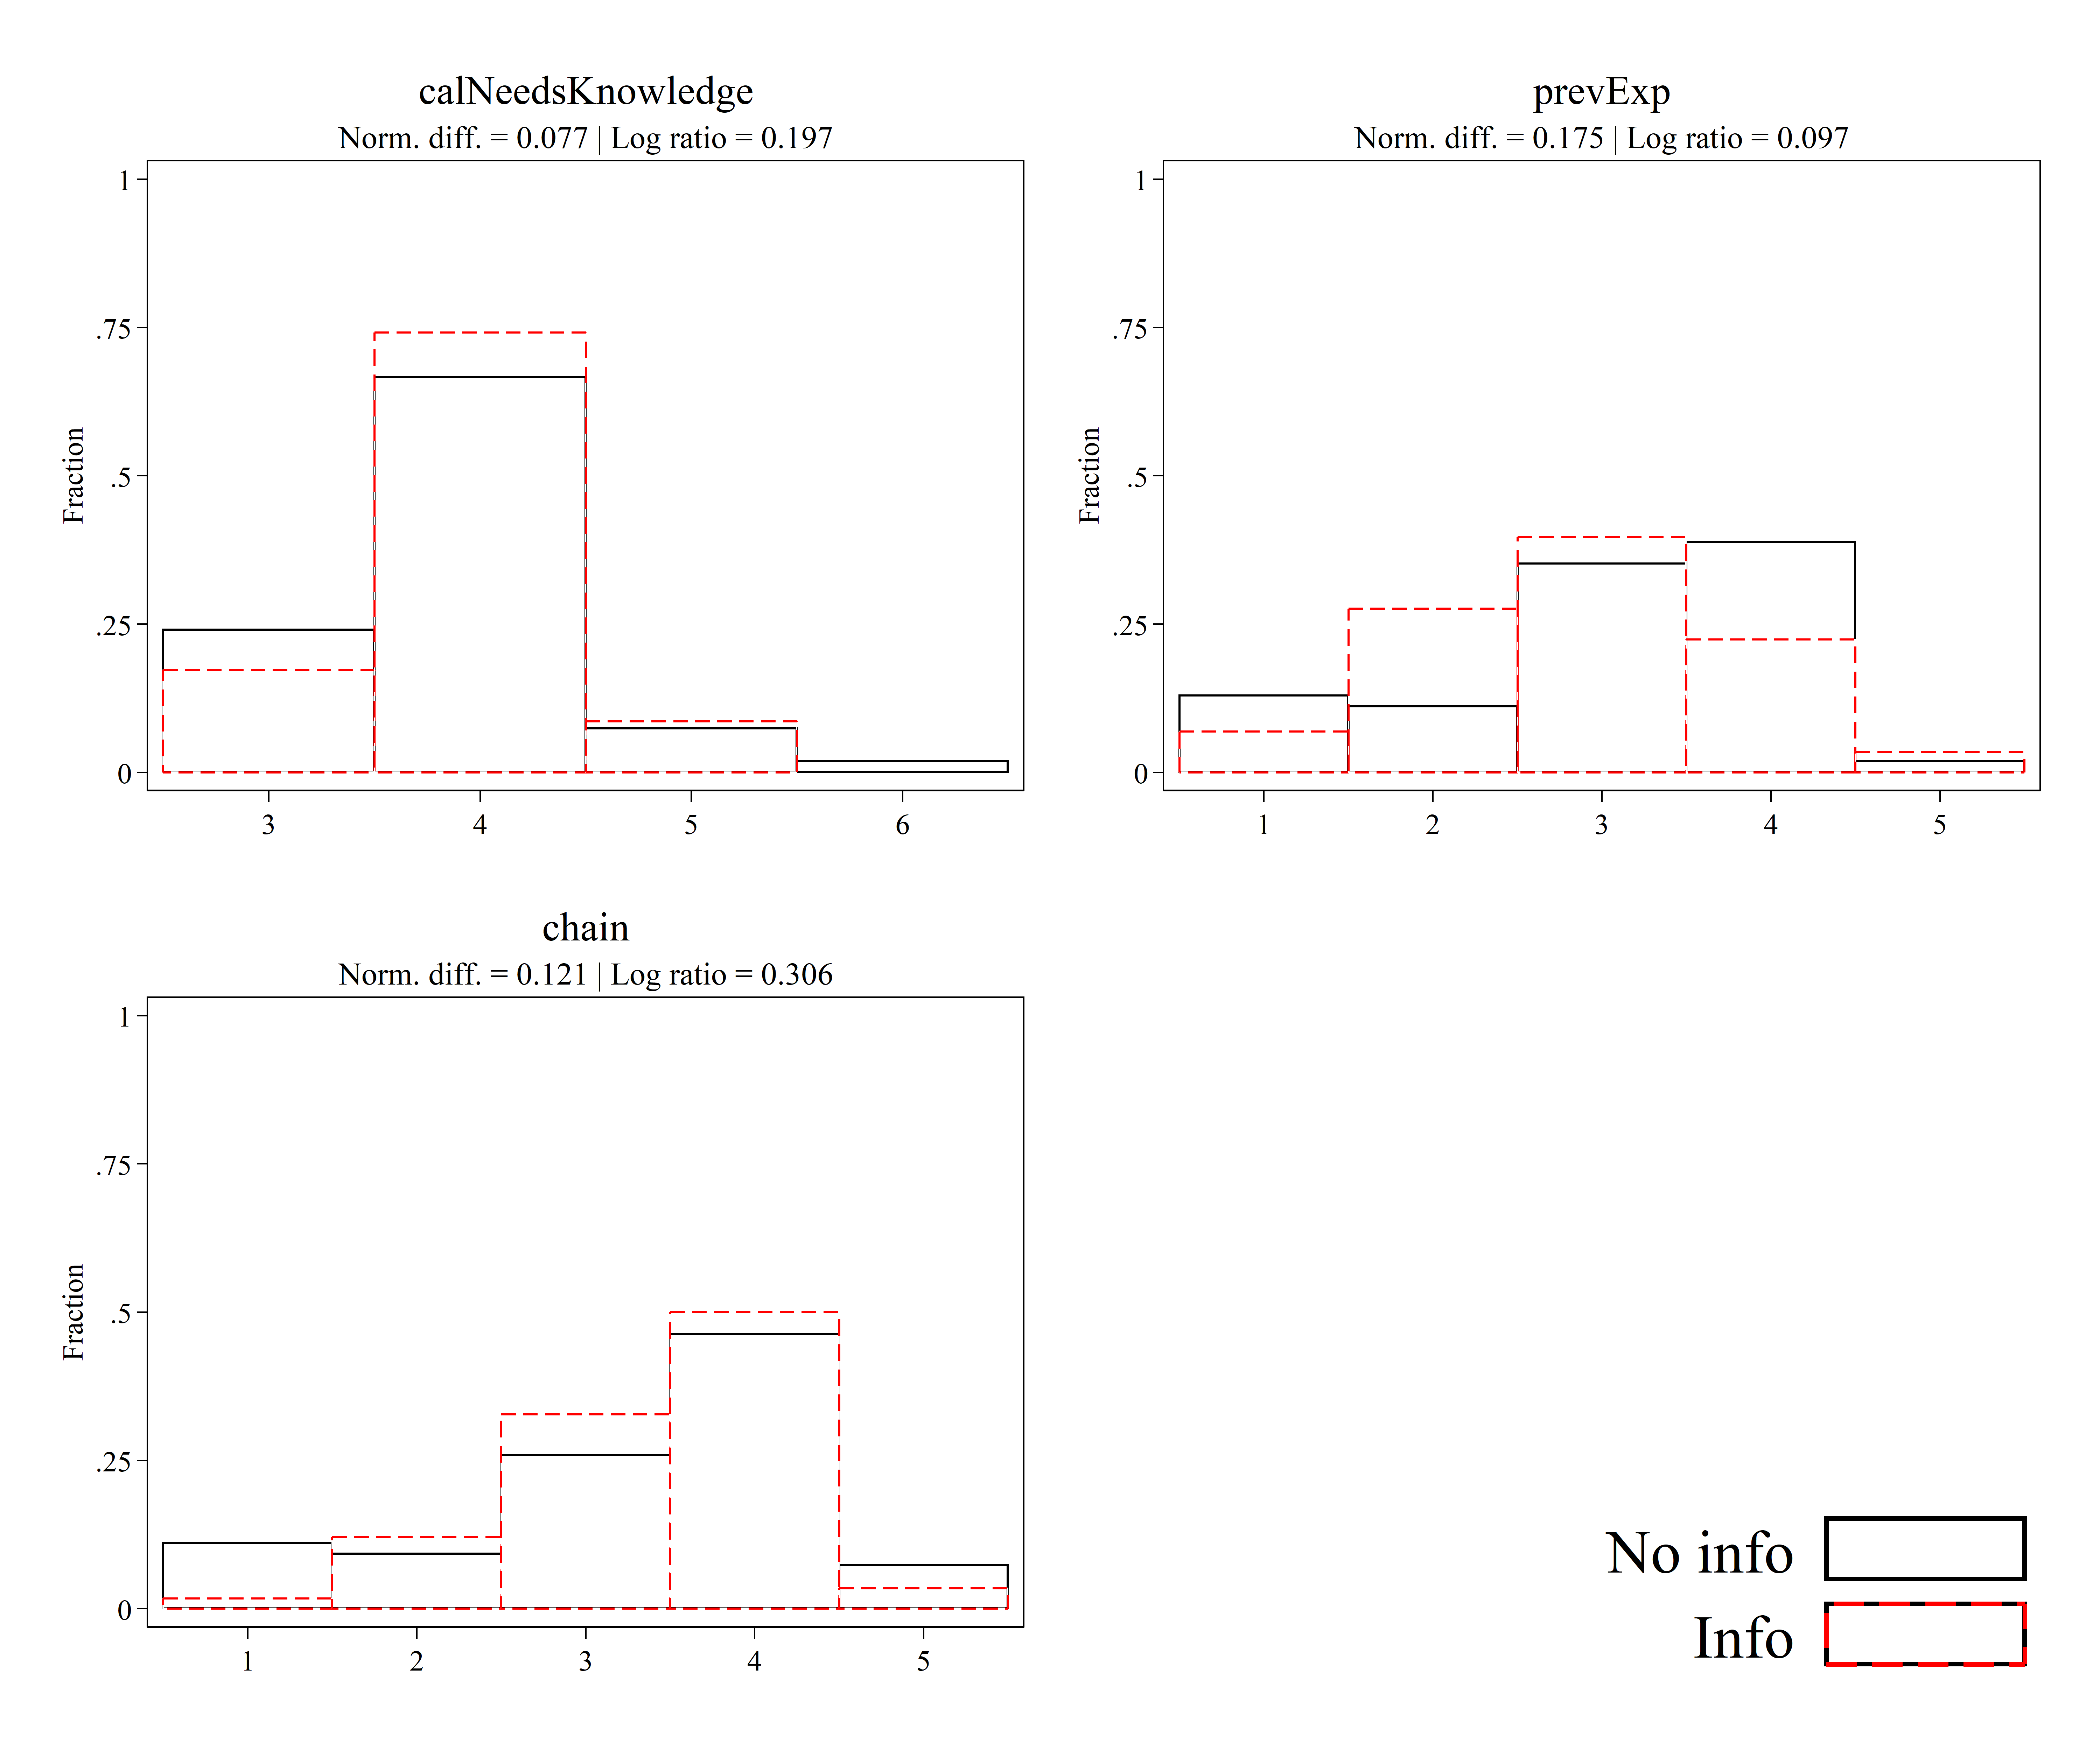
\includegraphics[width=1\textwidth]{./figures/covDifTreat_0_calorieKnow.png}}
  \end{center}
\end{figure}

\FloatBarrier

\clearpage


% ------------------------------------------------------------------------------
\section{Low baseline: group C vs group D}

Within participants who received a menu with calorie information for their hypothetical choices (high baseline, groups A and B): The group of participants who received a menu without calorie information for their real choice (group C) and the group of participants who received a menu with covered calorie information for their real choice (group D). The multivariate difference in normalized means is $1.19$.

\subsection{Demographics}

\begin{itemize}
  \item \textbf{Female}: No \emph{large} difference.

  \item \textbf{Age}: \emph{Large} difference.
  The normalized difference in means is 0.32 standard deviations and the normalized difference in variances is 0.39. Ths difference is not driven by outliers. After dropping them (value 39 in the no info group and values 44 and 46 in the info group), the normalized difference in means is 0.32 and the normalized difference in variances is 0.21.

  \item \textbf{College}: No \emph{large} difference.

  \item \textbf{Expenses}: \emph{Large} difference.
  Beyond the first two moments of the distribution, the histogram reveals differences in the lower end of the scale.

  \item \textbf{Income}: No \emph{large} difference.
  High log ratio driven by one outlier.

  \item \textbf{Weight description}: No \emph{large} difference.

  \item \textbf{BMI}: No \emph{large} difference.
\end{itemize}

\begin{figure}[ht]
  \caption{Balance in demographic characteristics \\ (group C vs D)}\label{fig:group3_demographics}
  \begin{center}
  {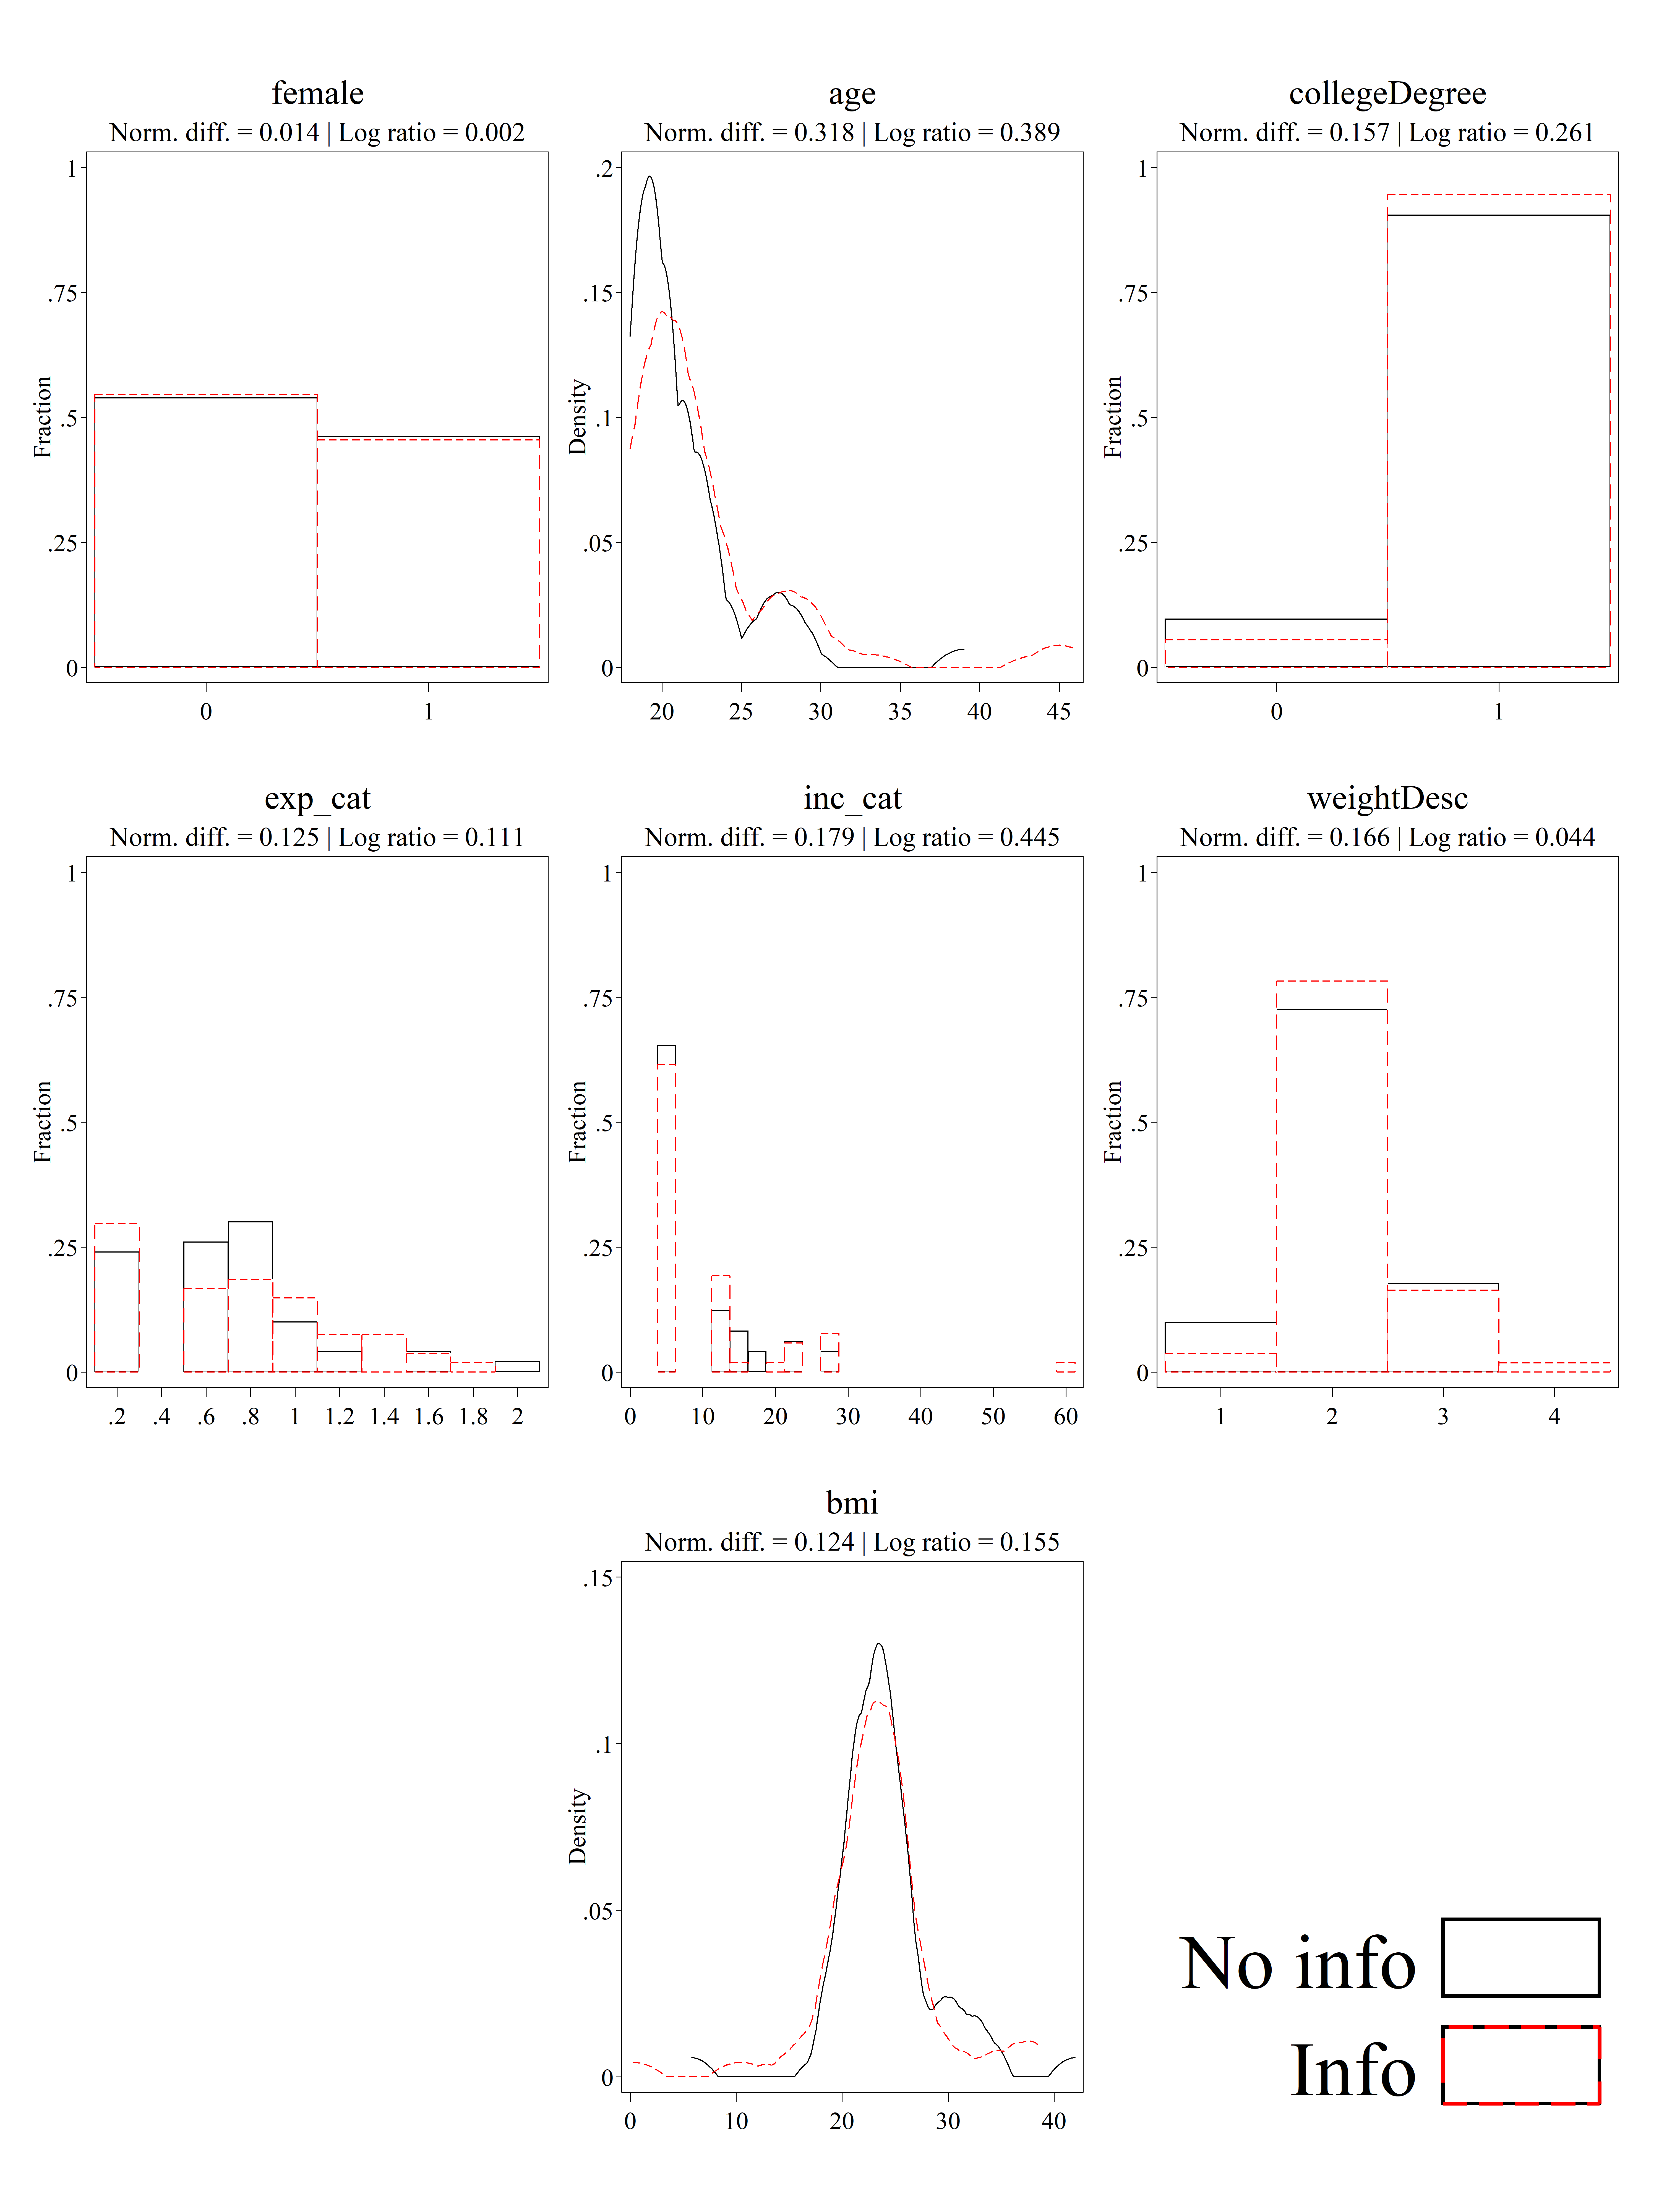
\includegraphics[width=1\textwidth]{./figures/covDifTreat_1_demographics.png}}
  \end{center}
\end{figure}

\FloatBarrier

\clearpage

\subsection{Attitudes}

\begin{itemize}
  \item \textbf{Risk preferences}: No \emph{large} difference.
  The normalized difference in means is 0.22, the normalized difference in variances is 0.06, and there are differences of 7.6 pp and 10 pp in the share of participants from each treatment arm in categories 4 and 3. However, the normalized difference in mean remains small because the treatment group with a higher share alternates in consecutive categories and offset each within-category difference.

  \item \textbf{Discount factor $\delta$}: No \emph{large} difference.

  \item \textbf{Present-bias $\beta$}: No \emph{large} difference.
  High normalized difference in means and variance is driven by one outlier most likey reflecting a mistake.

  \item \textbf{Food-self control}: No \emph{large} difference.
  The normalized difference in means is 0.17 and the normalized difference in variances is 0.14. In the kernel densities, the main difference comes from two outliers in the info group (values: 46, 50). Without these two outliers, the normalized difference in means is 0.06 and the normalized difference in variances is 0.1.

  \item \textbf{Hunger level}: \emph{Large} difference.
  The normalized difference in means is 0.36, the normalized difference in variances is 0.02, and the share of participants in the first two categories (i.e., less hungry) from the no info group exceeds the share from the info group by 13.8 percentage points. The inverse difference applies for the top two categories.
\end{itemize}

\begin{figure}[ht]
  \caption{Balance in demographic characteristics \\ (group A vs B)}\label{fig:group3_attitudes}
  \begin{center}
  {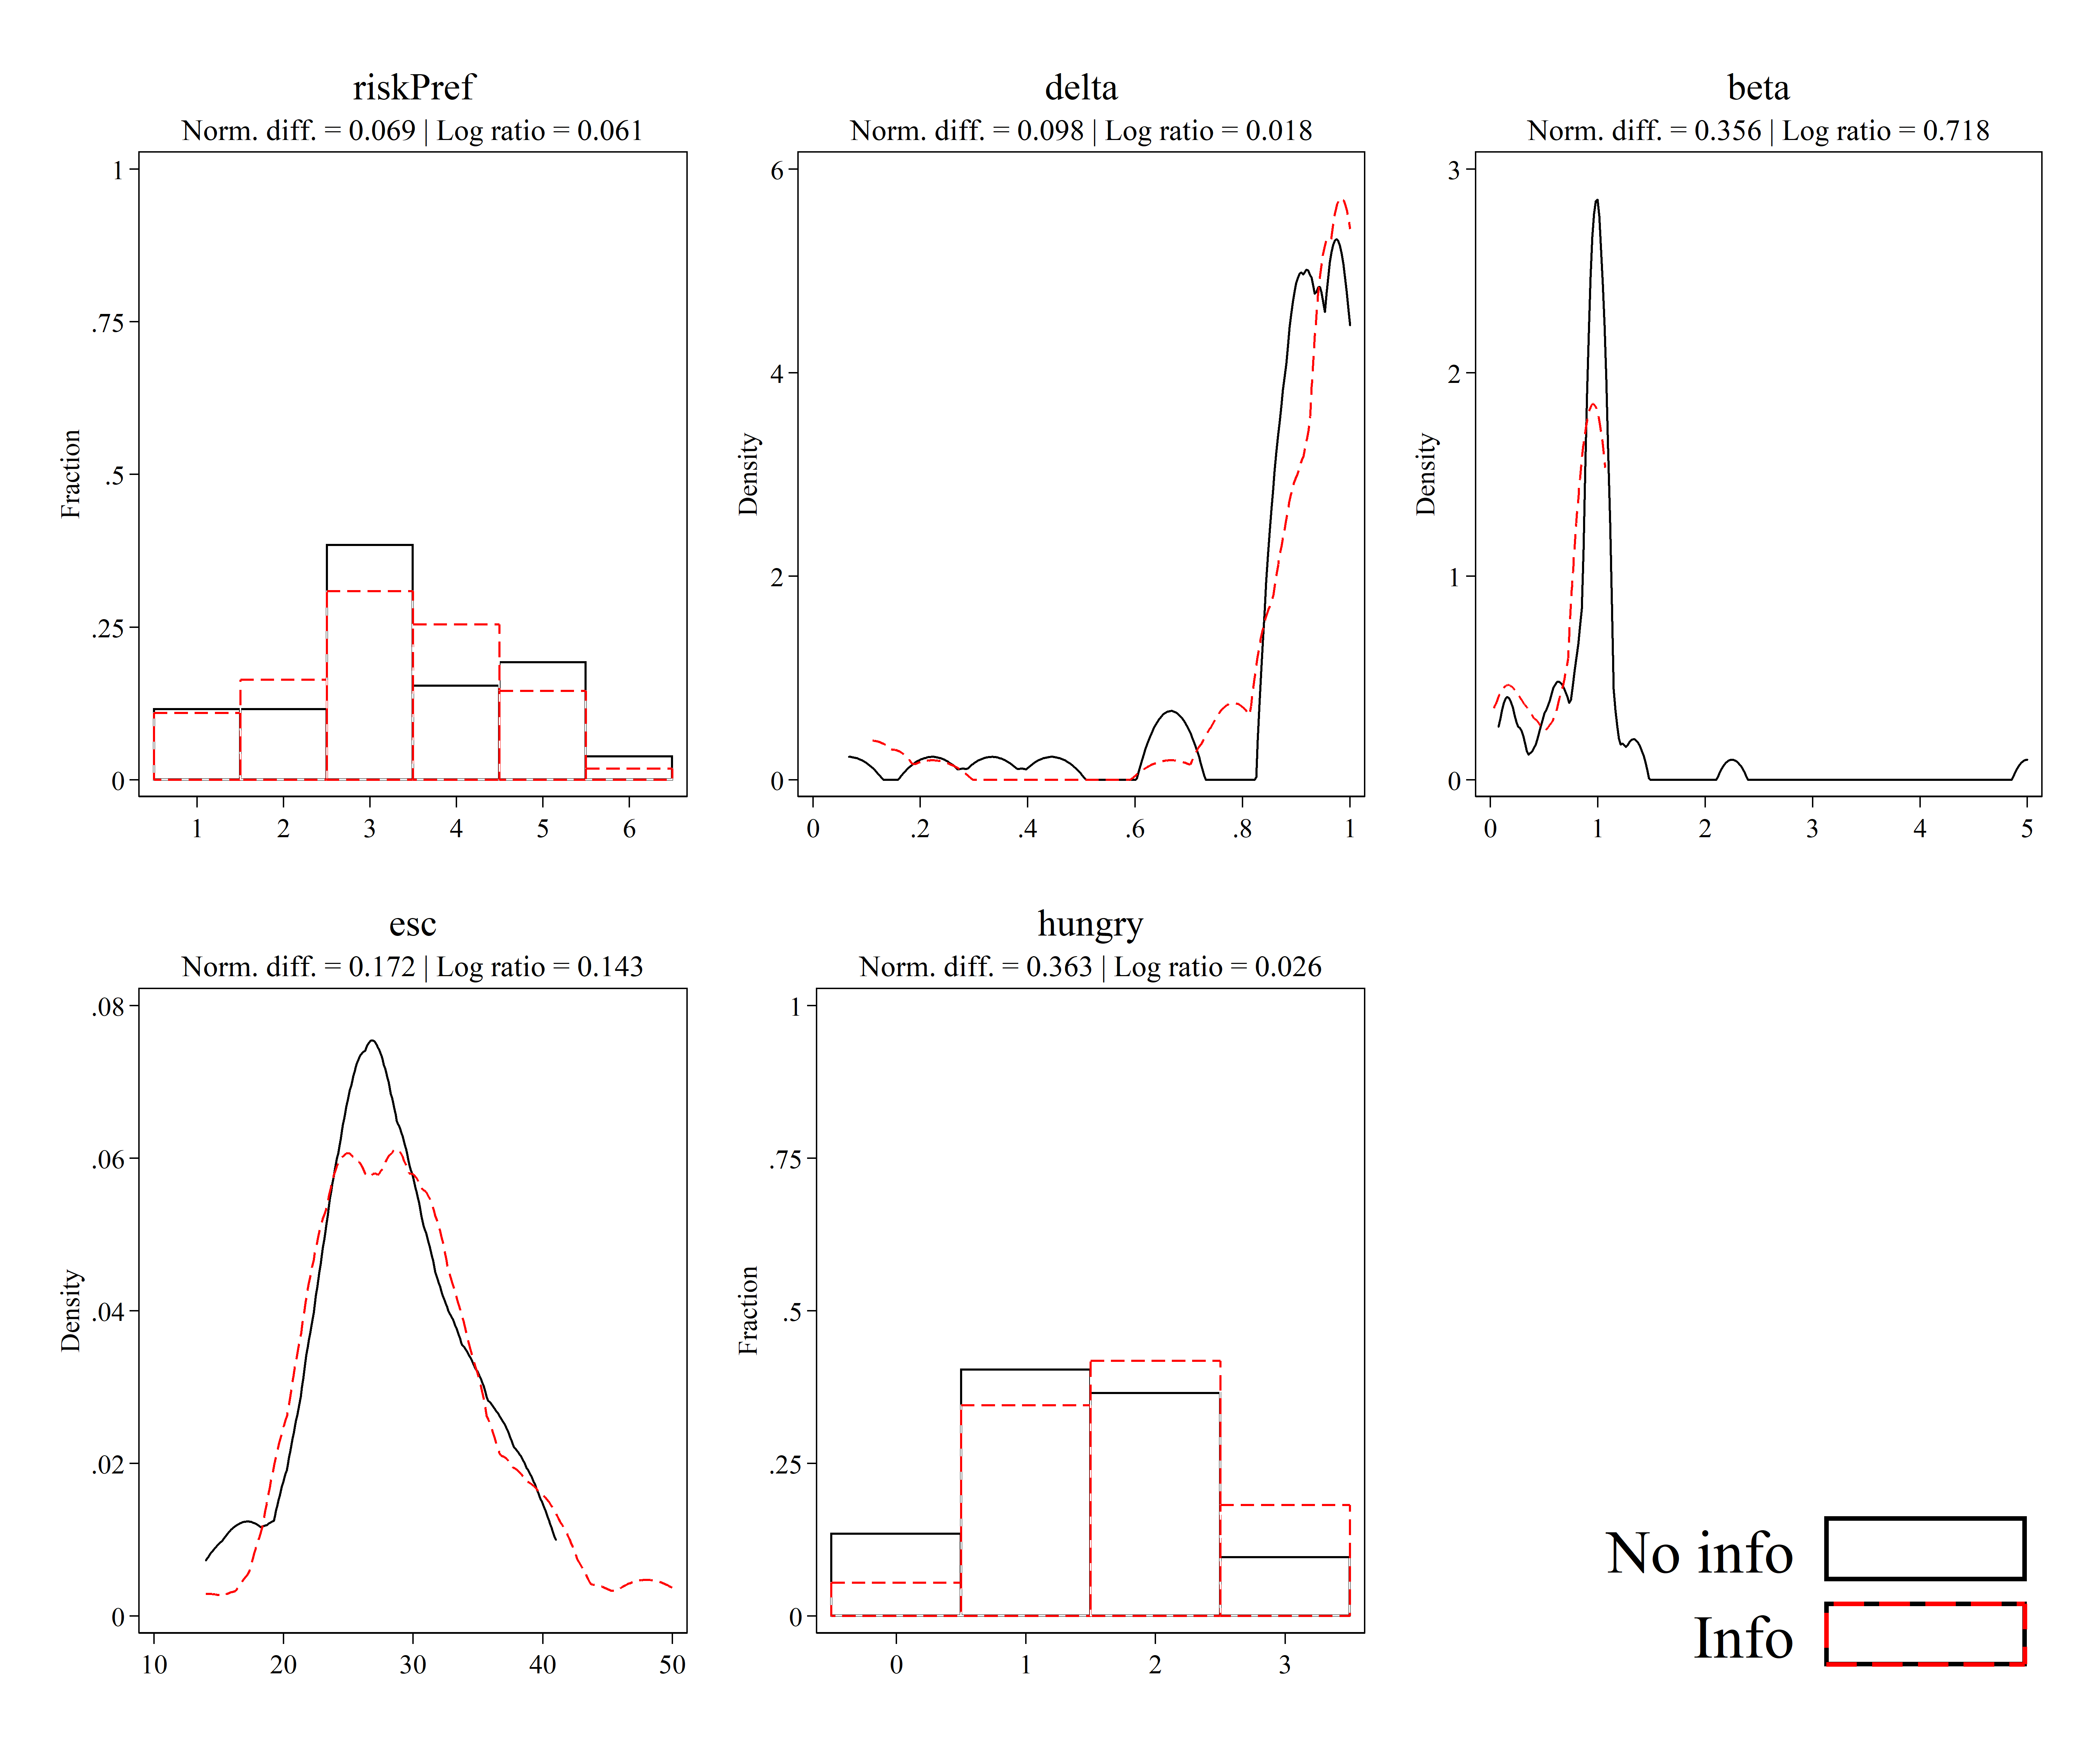
\includegraphics[width=1\textwidth]{./figures/covDifTreat_1_attitudes.png}}
  \end{center}
\end{figure}

\FloatBarrier

\clearpage

\subsection{Health status and perceptions}

\begin{itemize}
  \item \textbf{Health assessment}: \emph{Large} difference.

  \item \textbf{Would benefit from eating healthier}: No \emph{large} difference.

  \item \textbf{Wish could eat healthier at home}: No \emph{large} difference.

  \item \textbf{Wish could eat healthier out}: \emph{Large} difference.

  \item \textbf{Importance of eating healthy food}: No \emph{large} difference.

  \item \textbf{Importance of exercising regularly}: \emph{Large} difference.
  Beyond the normalized differences in means and variances, we identify this imbalance as \emph{large} because of the differences in the share responding 3 and 4. Regular exercise seems less important for those in the endowed group.

  \item \textbf{Importance of healthy body weight}: \emph{Large} difference.
\end{itemize}

\begin{figure}[ht]
  \caption{Balance in demographic characteristics \\ (groups A and B vs groups C and D)}\label{fig:group3_health}
  \begin{center}
  {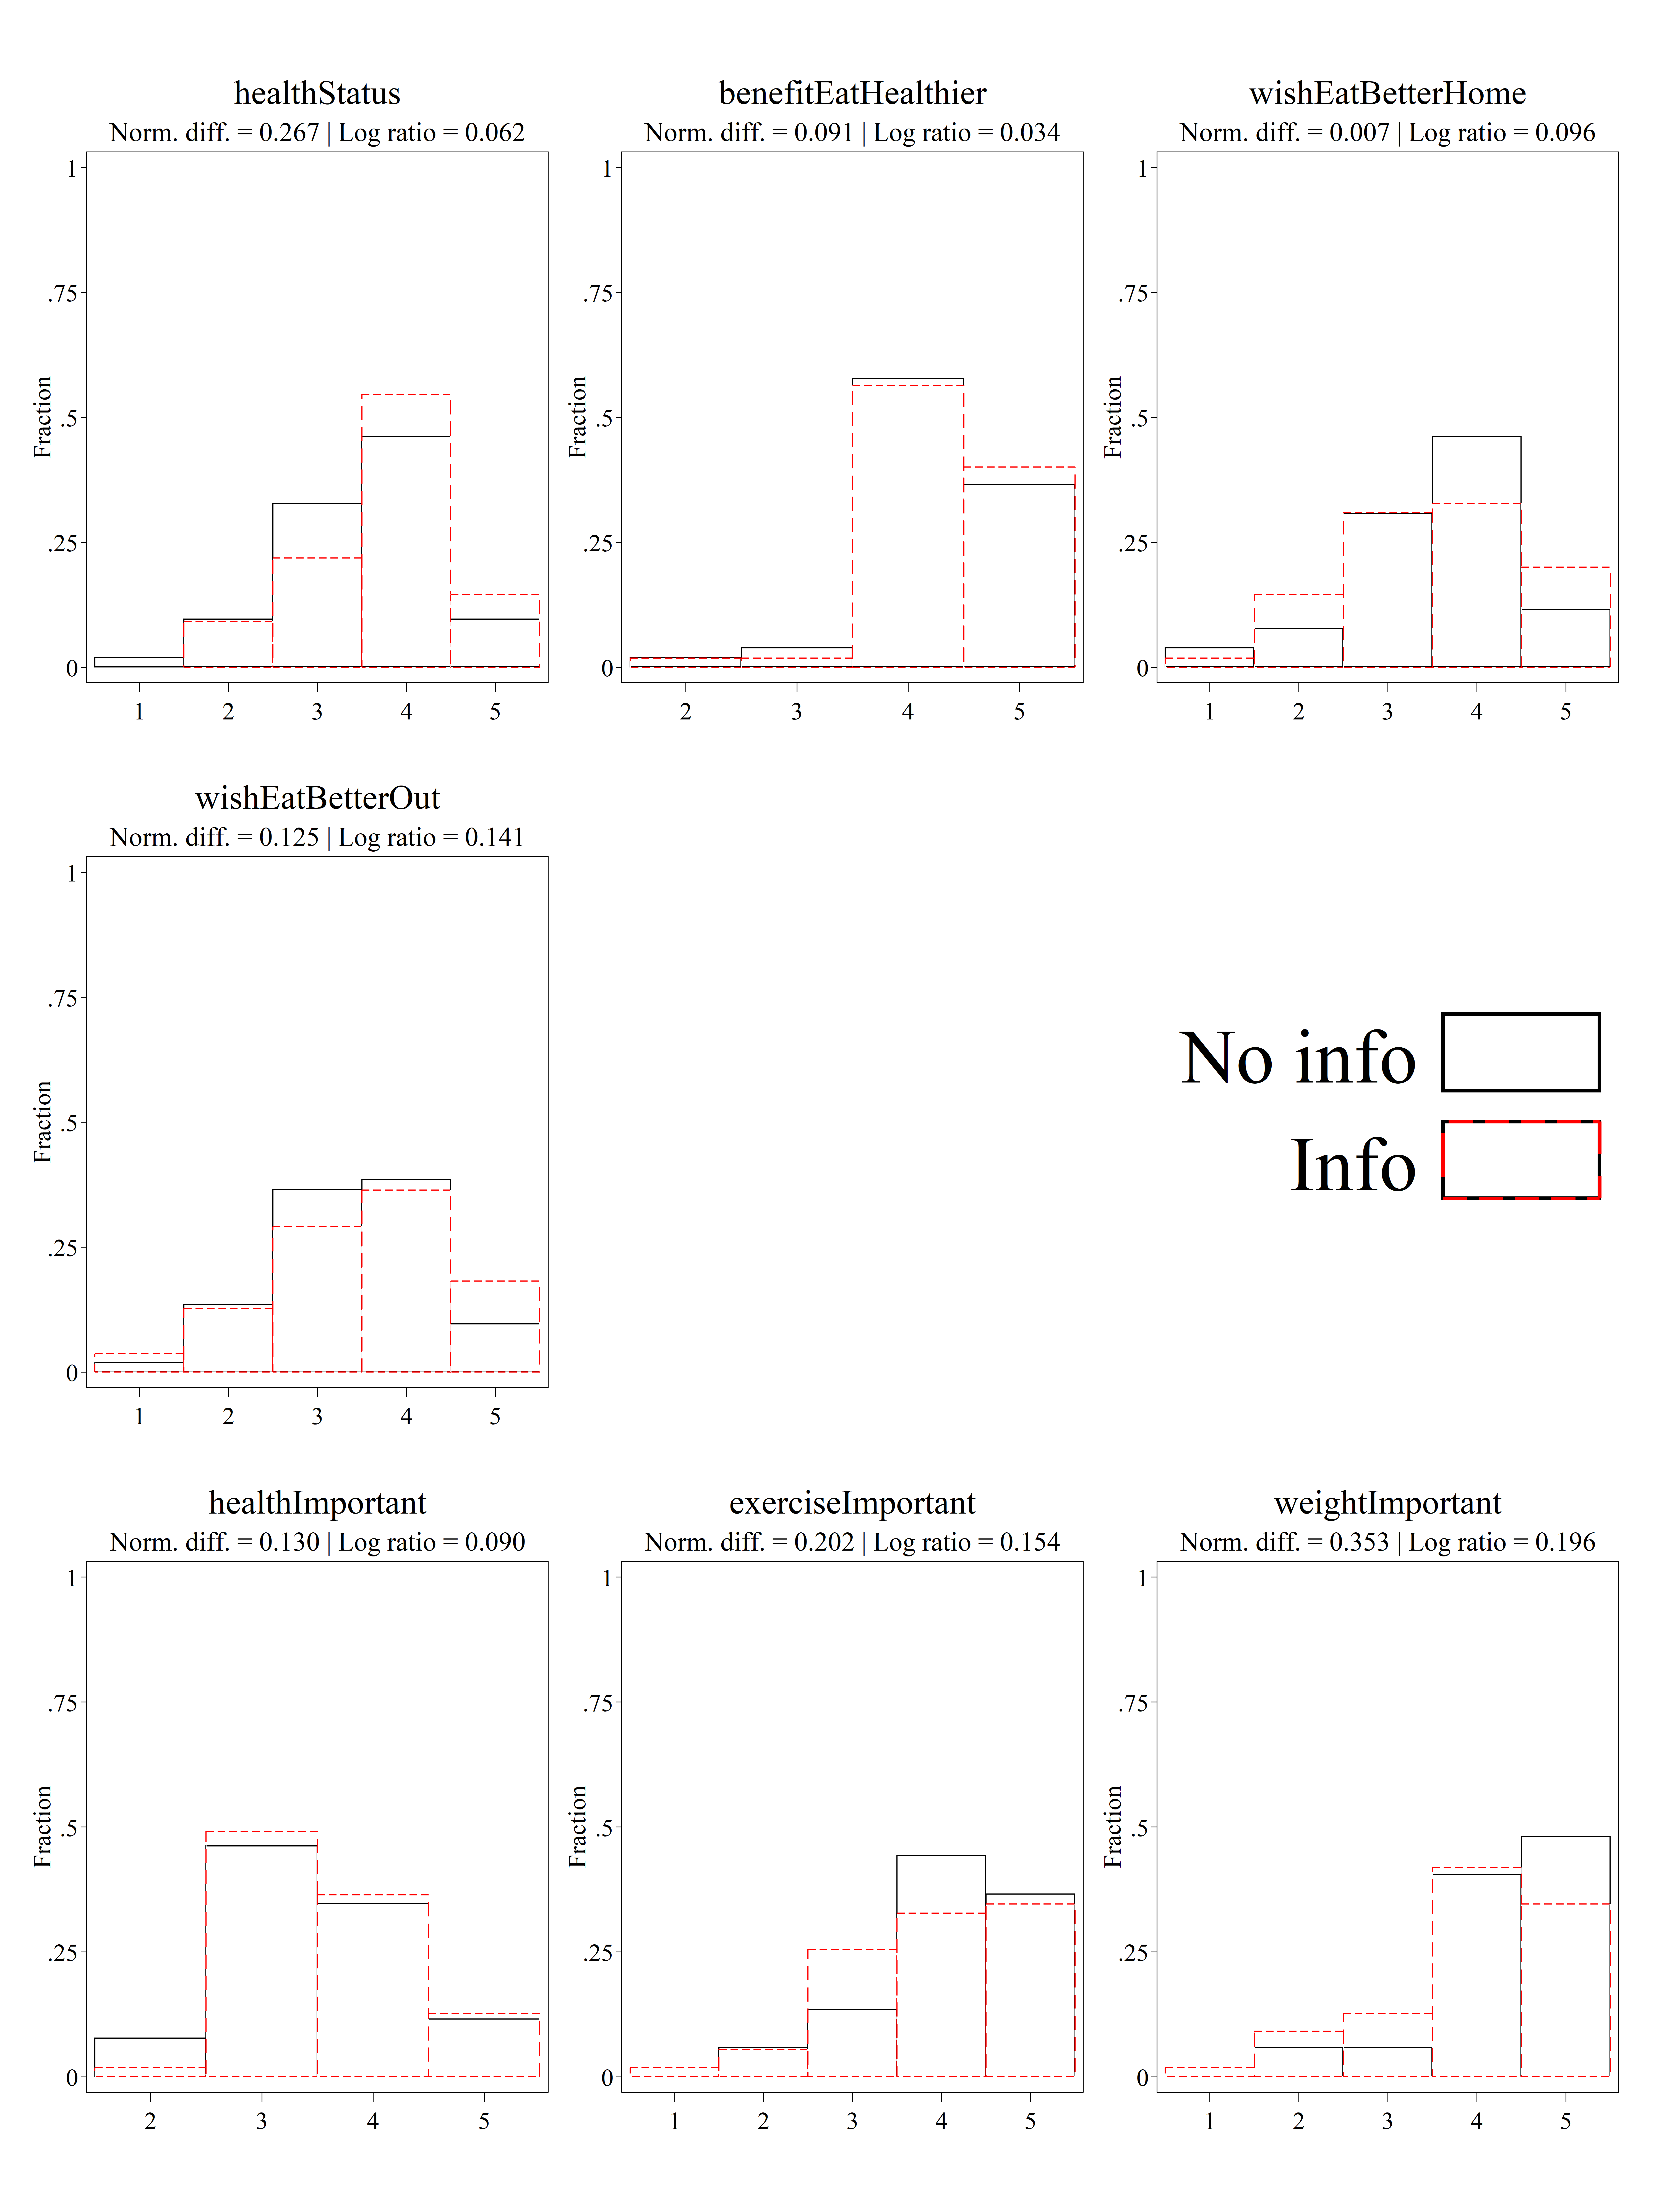
\includegraphics[width=1\textwidth]{./figures/covDifTreat_1_health.png}}
  \end{center}
\end{figure}

\FloatBarrier

\clearpage

\subsection{Knowledge of calorie information}

\begin{itemize}
  \item \textbf{Knows calorie needs}: \emph{Large} difference.

  \item \textbf{Experience with calorie information}: \emph{Large} difference.
  The normalized difference in means is 0.13 and the normalized difference in variances is 0.07. However, there are large differences within categories. Even if the treatment arms alternate the higher share in consecutive categories – offsetting each other and resulting in a small normalized difference in means –, we consider the difference \emph{large}.

  \item \textbf{Frequency visits to chain restaurants}: \emph{Large} difference.
  Those in the endowed group seem to visit chain restaurants more often (it is mandated to show calories in those restaurants).
\end{itemize}

\begin{figure}[ht]
  \caption{Balance in demographic characteristics \\ (group C vs D)}\label{fig:group3_calorie}
  \begin{center}
  {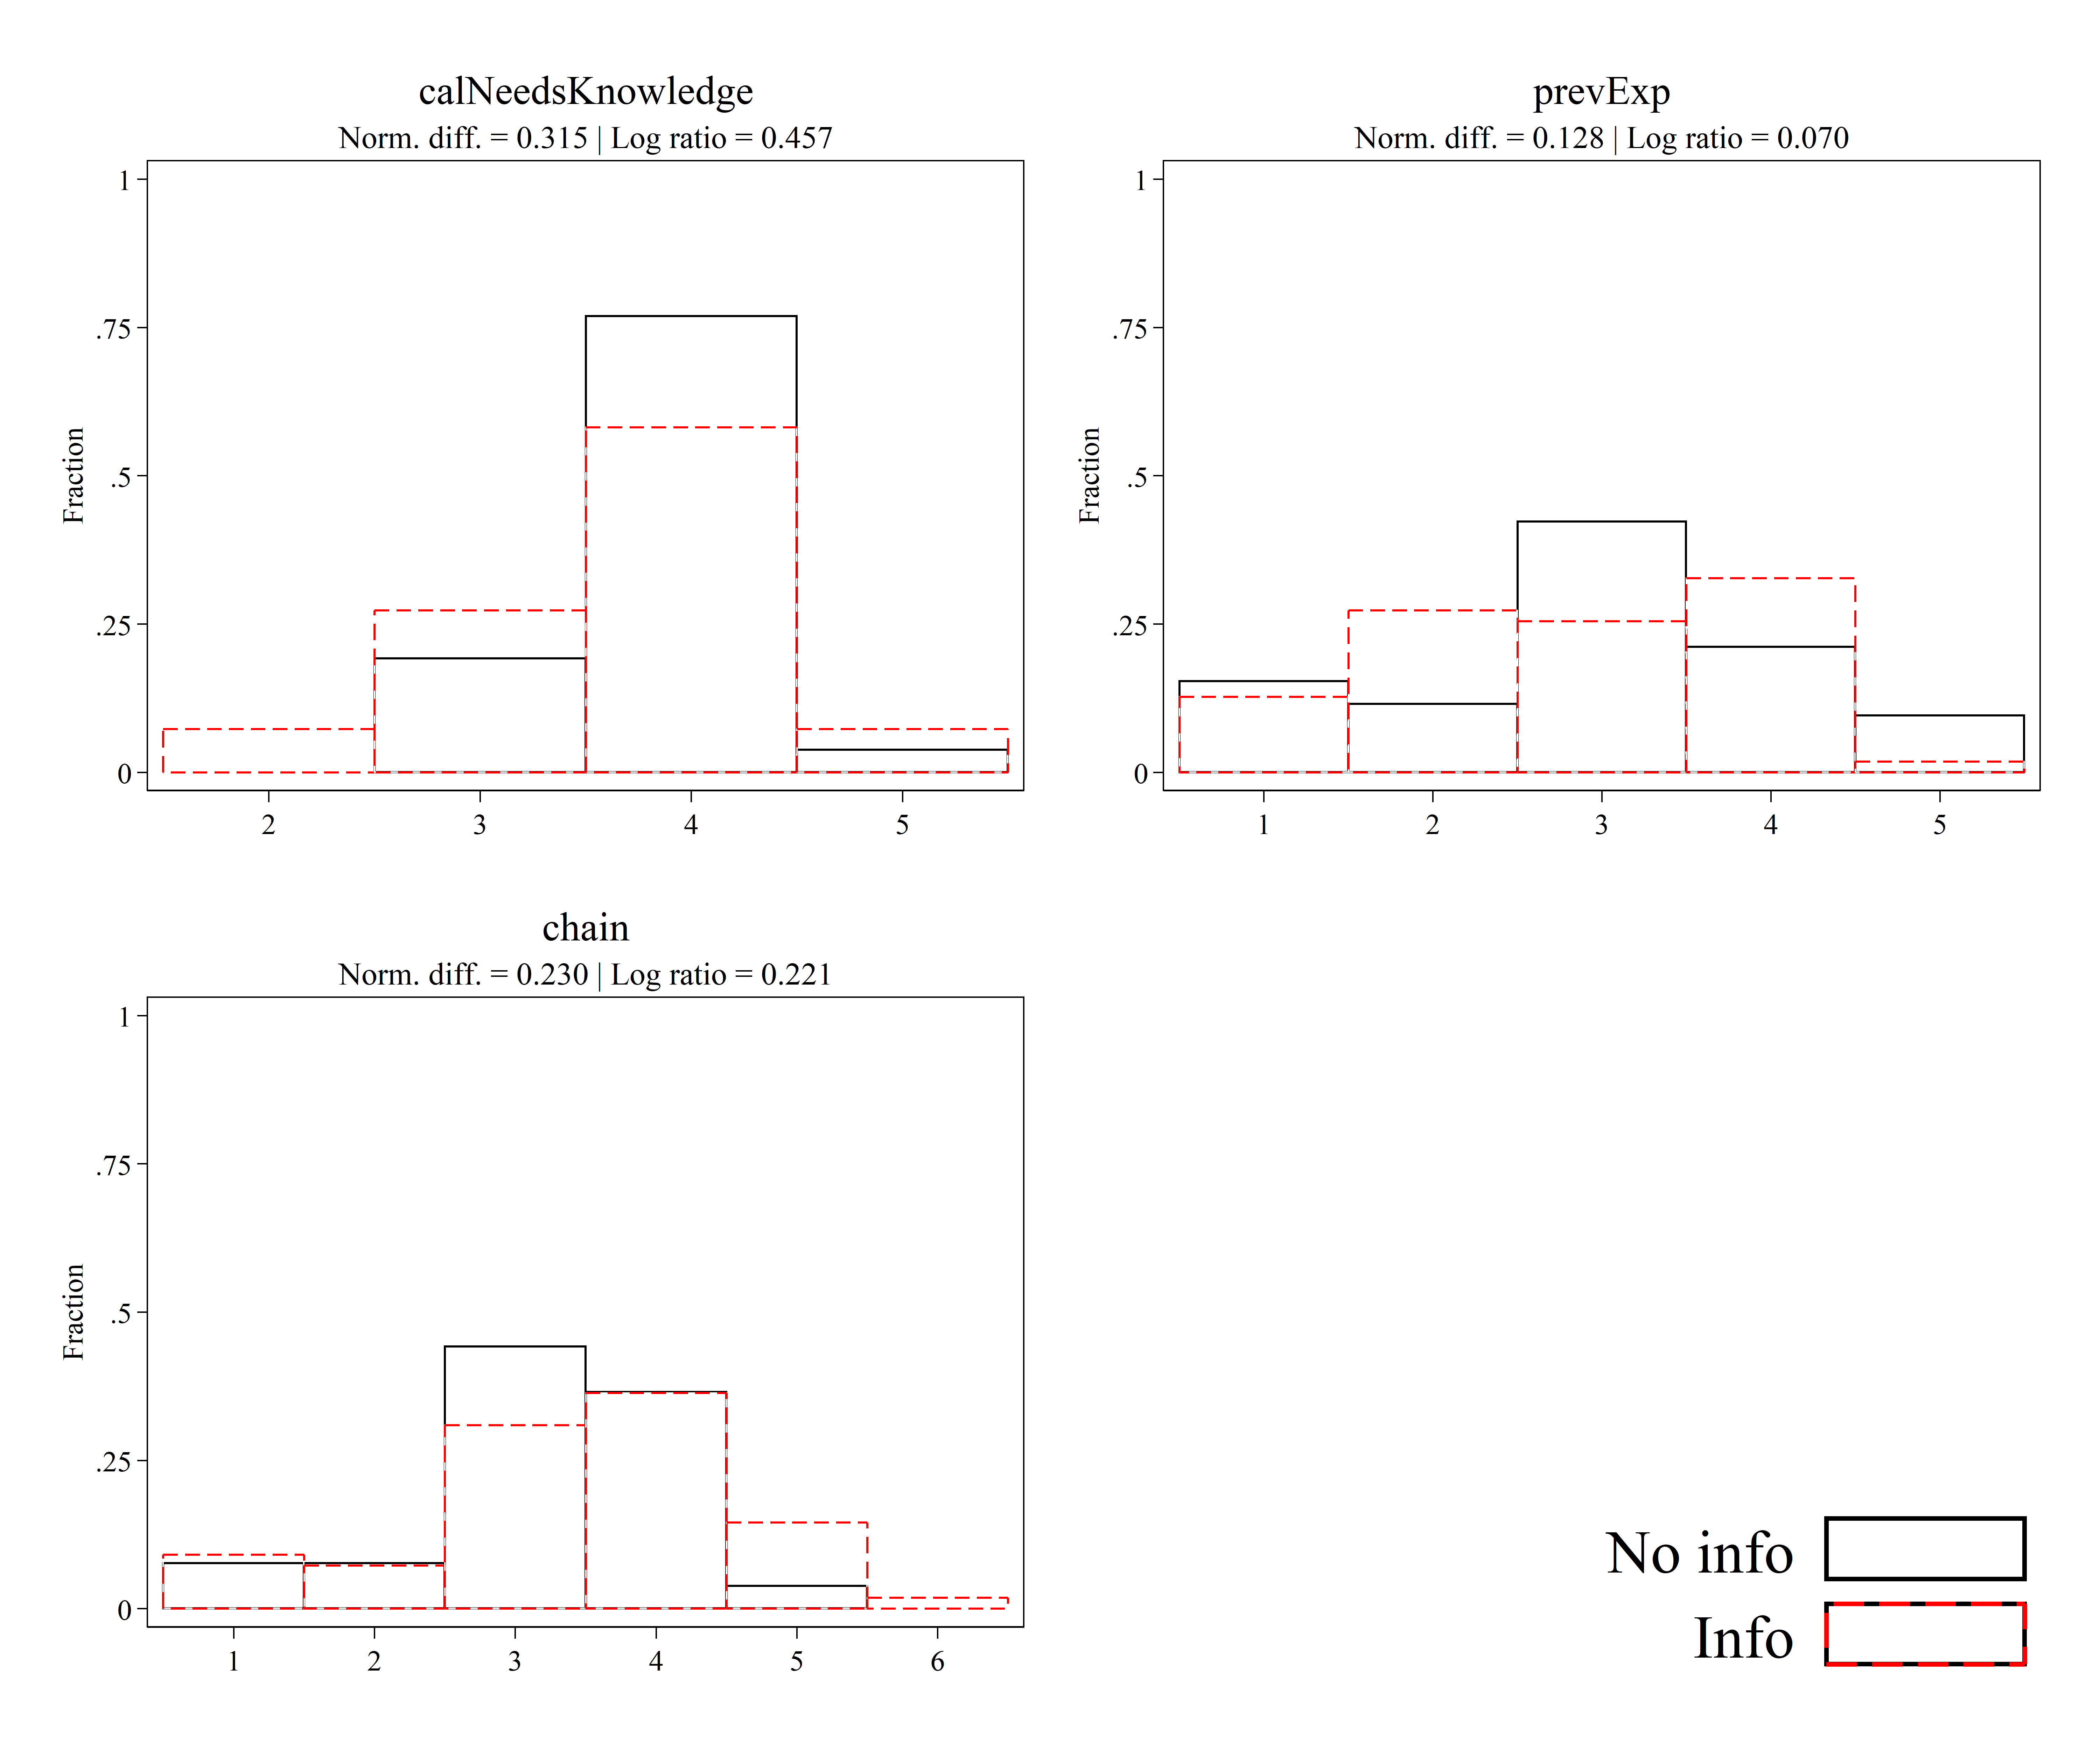
\includegraphics[width=1\textwidth]{./figures/covDifTreat_1_calorieKnow.png}}
  \end{center}
\end{figure}

\FloatBarrier

\end{document}
